%********************************************************************************
\documentclass{article}


\usepackage{appendix}
\usepackage{natbib}
\bibliographystyle{abbrvnat}
\bibpunct{(}{)}{;}{a}{,}{,}
\usepackage{setspace}
\usepackage{amsmath}
\usepackage{amsfonts}
\usepackage{amsthm}
\usepackage{amssymb}
%\newtheorem{assumption}{Assumption}
\newtheorem{proposition}{Proposition}
\usepackage{booktabs}
\usepackage[usenames, dvipsnames]{color}
\usepackage{epsfig}
\usepackage{epstopdf}
\usepackage{graphics}
\usepackage{hyperref}
\usepackage{lscape}
\usepackage[capposition=top]{floatrow}
\usepackage{subcaption}
\usepackage{subfloat}



\newcommand{\sdidloc}{./../../spillovers}
\newcommand{\JELs}{\hspace{8mm} \emph{JEL codes}: C13, C21, J13, R23. \\}

\hypersetup{
    colorlinks=true,      
    linkcolor=BlueViolet, 
    citecolor=BlueViolet, 
    filecolor=BlueViolet, 
    urlcolor=BlueViolet   
}

\setlength\parskip{0.25in}
\setlength\topmargin{-0.375in}
\setlength\textheight{8.8in}
\setlength\textwidth{5.8in}
\setlength\oddsidemargin{0.4in}
\setlength\evensidemargin{-0.5in}


\newtheorem*{assumption*}{\assumptionnumber}
\providecommand{\assumptionnumber}{}
\makeatletter
\newenvironment{assumption}[2]
 {%
  \renewcommand{\assumptionnumber}{Assumption #1{#2}}%
  \begin{assumption*}%
  \protected@edef\@currentlabel{#1}%
 }
 {%
  \end{assumption*}
 }
\makeatother
\newcommand{\asref}[2]{\ref{#1}{\textcolor{BlueViolet}{#2}}}


\newcommand{\Var}{\mathrm{Var}}
\newcommand{\Cov}{\mathrm{Cov}}
\newcommand{\Bias}[2]{\frac{\Cov[#1,#2]}{\Var[#1]}}


%ABSTRACT WITHIN CHAPTER
\usepackage{changepage}%
\makeatletter
\newenvironment{chapabstract}{%
    \begin{center}%
      \bfseries Abstract
    \end{center}}%
   {\par}
\makeatother
\newif\ifheading



%\title{\textbf{Estimating Difference-in-Differences in the Presence of Spillovers: 
%Theory and Application to Contraceptive Reforms in Latin America}
\title{Estimating Difference-in-Differences in the Presence of Spillovers\thanks{
I thank participants in the Impact Evaluation Meeting at the Inter-American 
Development Bank for useful comments on this draft. Full source code, including the
Stata module \texttt{cdifdif} is available for download and use at 
\href{https://github.com/damiancclarke/spillovers}{https://github.com/damiancclarke/spillovers}.  
Affiliation: Faculty of Economics, Universidad de Santiago de Chile. Contact email:
\href{mailto:damian.clarke@usach.cl}{damian.clarke@usach.cl}}}
\author{Damian Clarke}
\date{August, 2015}

\begin{document}
\maketitle
\begin{spacing}{1.3}
\begin{chapabstract}
I propose a method for difference-in-differences (DD) estimation in situations 
where the stable unit treatment value assumption is violated locally. This is
relevant for a wide variety of cases where spillovers may occur between quasi-%
treatment and quasi-control areas in a (natural) experiment. A flexible 
methodology is described to test for such spillovers, and to consistently 
estimate treatment effects in their presence. This methodology is illustrated
using two recent examples of contraceptive reform.  It is shown that with both
the arrival of abortion to Mexico DF, as well as the arrival of the emergency
contraceptive pill to certain areas of Chile, reductions in teenage pregnancy
occurred in both reform neighbourhoods as well as nearby (but theoretically
untreated) neighbourhoods.  Where reforms are geographically disperse, I 
demonstrate that spillovers can cause considerable concern regarding the 
unbiasedness of the traditional DD estimates widely employed in the economic 
literature. %Applying this methodology provides considerable insight into
%the estimation of the impact of contraceptive reform on teenage pregancy: a 
%topical and important policy issue for governments in Latin America.
\end{chapabstract}
\JELs
\newpage
%================================================================================
\section{Introduction}
Natural experiments often rely on territorial borders to estimate treatment 
effects.  These borders separate quasi-treatment from quasi-control groups with
individuals in one area having access to a program or treatment while those in 
another do not.  In cases such as these where geographic location is used to 
motivate identification, the stable unit treatment value assumption (SUTVA) is, 
either explicitly or implicitly, invoked.\footnote{The SUTVA has a long and 
interesting history, under various guises. \citet{Cox1958} refers to ``no 
interference between different units'', before \citet{Rubin1978} introduced the 
concept of SUTVA (the name SUTVA did not appear until \citet{Rubin1980}).  
Recent work of \citet{Manski2013}, refers to this assumption as Individualistic 
Treatment Response (ITR).}

However, often territorial borders are porous.  Generally state, regional,
municipal, and village boundaries can be easily, if not costlessly, crossed.
Given this, researchers interested in using natural experiments in this way may
be concerned that the effects of a program in a treatment cluster may spillover 
into non-treatment clusters---at least locally.

Such a situation is in clear violation of the SUTVA's requirement that the 
treatment status of any one unit must not affect the outcomes of any other unit.  
In this paper I propose a methodology to deal with such spillover effects.  I
discuss how to test for local spillovers, and if such spillovers exist, how to 
estimate unbiased treatment effects in their presence.  It is shown that this 
estimation requires a weaker condition than SUTVA: namely that SUTVA holds 
between \emph{some} units, as determined by their distance from the treatment 
cluster.  I show how to estimate treatment and spillover effects, and then
propose a method to generalise the proposed estimator to a higher dimensional 
case where spillovers may depend in a flexible way on an arbitrary number of 
factors.

It is shown that this methodology recovers unbiased treatment estimates under 
quite general violations of SUTVA.  While it is assumed that the distance of 
an individual to the nearest treatment cluster determines whether stable unit 
treatment type assumptions hold for that individual, `distance' is defined 
very broadly.  It is envisioned that this will allow for phenomena such as 
information flowing from treated to untreated areas, or of untreated 
individuals violating their treatment status by travelling from untreated to
treated areas.  In each case distance plays a clear role in the propogation 
of treatment; either information must travel out, or beneficiaries must travel 
in. Similarly, this framework allows for local general equilibrium-type 
spillovers, where a tightly applied program may have an economic effect on 
nearby markets, but where this effect disipates as distance to treatment 
increases.

Turning to empirics, this methodology is illustrated with two examples.
I examine how spillovers of reforms across municipal boundaries may 
contaminate `traditional' difference-in-differences (DD) estimators.  This is 
applied to two contraceptive reforms where individuals from contiguous or nearby 
areas can travel to a treatment region to access the reform.  It is shown that 
both the arrival of the morning after pill to certain municipalities of Chile, 
and abortion to certain districts in Mexico, results in a reduction of births in 
the given area, as well as in close-by quasi-control areas.  As a result, the 
spillover-robust DD estimator propsed here flexibly captures this effect, 
correcting for any (local) spillover bias that traditional DD fails to 
identify.  The choice of empirical example: contraceptive reform in Latin America,
is not casual.  I illustrate spillovers in Latin America, firstly, given the
importance of correctly estimating the effect sizes of reforms in this context.
Latin America is a region with high rates of adolescent pregnancy, second only to 
Sub-Saharan Africa world-wide (see appendix figure \ref{SFig:continents}).  Within 
Latin America, countries have had varying success in curbing these very high rates 
(figure \ref{SFig:countries}).  Secondly, the costs of undesired pregnancy are very 
high, resulting in considerable incentives to travel to receive access to contraception
or abortion if available in other areas.  Taken together, these stylised facts 
suggest that the analysis of contraceptive reform is both of importance to 
policy makers, and also potentially particularly likely to suffer from the shortfalls 
of traditional DD estimation.

Although in both these examples distance is a geographic measure, calculated
variously as Euclidean distance, shortest distance over roads, and shortest 
travel times between areas, this methodology should not be considered as limited 
to spatial spillovers.  Univariate measures of distance including propogation 
through nodes in a network, ethnic distance, ideological distance, or other 
quantifiable measures of difference between units can be used in precisely the 
same manner.  I also show how multivariate measures of distance, or interactions 
between distance and other variables, can be similarly employed.  This is 
particularly useful for cases where the effects of spillovers may be expected to 
vary by individual characteristics such as age, socioeconomic status, access to 
transport or access to information.

This paper joins recent literature which aims to loosen the strong structure 
imposed by the SUTVA.  Perhaps most notably, it is (in broad terms) an 
application of \citeauthor{Manski2013}'s (2013) social interactions framework, 
focusing on the case where spillovers are restricted to areas local to treatment 
clusters.  However, unlike recent developments focusing on spillovers 
between treated and control units \emph{within} a treatment cluster (notable
examples include \citet{McIntosh2008,Bairdetal2014,AngelucciDiMaro2010}), this 
paper focuses on situations where entire clusters are treated, and the status
of the \emph{cluster} may affect nearby non-treated clusters.  This is likely
the case for quasi-experimental studies, where `experiments' are defined based
on geographic boundaries, such as administrative political regions which set 
different policies.\footnote{A very different case is that of (for example)
PROGRESA/Oportunidades, where treatment clusters (ie localities or 
\emph{localidades}) contained both treatment and control individuals, and the
literature is concerned with spillovers between treatment and control individuals
within this treatment cluster.}

\nocite{AngelucciDeGiorgi2009} \nocite{Heckmanetal1998}
\nocite{MiguelKremer2004}
 \nocite{Heckmanetal1998b}

%================================================================================
\section{Methodology}
Define $Y(i,t)$ as the outcome for individual $i$ and time $t$.  The population
of interest is observed at two time periods, $t\in \{0,1\}$. Assume that between
$t=0$ and $t=1$, some fraction of the population is exposed to a 
quasi-experimental treatment.  As per \citet{Abadie2005}, I will denote 
treatment for individual $i$ in time $t$ as $D(i,t)$, where $D(i,1)=1$ implies 
that the individual was treated, and $D(i,1)=0$ implies that the individual was
not directly treated.  Given that treatment only exists between periods 0 and 1,
$D(i,0)=0\ \forall\ i$.

It is shown by \citet{AshenfelterCard1985} that if the outcome is generated by
a component of variance process:
\begin{equation}
\label{Seqn:COV}
Y(i,t)=\delta(t) + \alpha D(i,t)+\eta(i)+\nu(i,t)
\end{equation}
where $\delta(t)$ refers to a time-specific component, $\alpha$ as the impact of 
treatment, $\eta(i)$ a component specific to each individual, and $\nu(i,t)$ as 
a time-varying individual (mean zero) shock, then a sufficient condition for 
identification (a complete derivation is provided by \citet{Abadie2005}) is:
\begin{equation}
\label{Seqn:ID}
P(D(i,1)=1|\nu(i,t))=P(D(i,1)=1) \ \forall\ t\in\{0,1\}.
\end{equation}
In other words, identification requires that selection into treatment does not
rely on the unobserved time-varying component $\nu(i,t)$.  If this condition 
holds, then the classical DD estimator provides an unbiased estimate of the
treatment effect:
\begin{equation}
\label{Seqn:DD}
\begin{split}
\alpha&=\{E[Y(i,1)|D(i,1)=1]-E[Y(i,1)|D(i,1)=0]\} \\
      &-\{E[Y(i,0)|D(i,1)=1]-E[Y(i,0)|D(i,1)=0]\}
\end{split}
\end{equation}
where $E$ is the expectations operator.

Assume now, however, that treatment is not precisely geographically bounded.  
Specifically, I propose that those living in control areas `close to' treatment 
areas are able to access treatment, either partially or completely.  Such a 
case allows for a situation where individuals `defy' their treatment status, by 
travelling or moving to treated areas, or where spillovers from treatment 
areas is diffused through general equilibrium processes.  Define $R(i,t)$ 
where:
\begin{equation}
\nonumber
 R(i,t) =
  \begin{cases}
   f\Big(X(i,t)\Big)>0   & \text{if an individual resides close to, but not in, a treatment area} \\
   0                            & \text{otherwise} 
  \end{cases}
\end{equation}
Where $X(i,t)$ is an individual covariate measuring distance (in a very general 
sense) to treatment and $f(\cdot)$ is a positive monotone function. As treatment 
occurs only in 
period 1, $R(i,0)=0$ for all $i$.  Similarly, as living in a treatment area 
itself excludes individuals from living `close to' the same treament area, 
$R(i,t)=0$ for all $i$ such that $D(i,t)=1$.

Generalising from (\ref{Seqn:COV}), now I assume that $Y(i,t)$ is generated 
by:
\begin{equation}
\label{Seqn:COV2}
Y(i,t)=\delta(t) + \alpha D(i,t)+\beta R(i,t)+\eta(i)+\nu(i,t)
\end{equation}
If we observe only $Y(i,t)$, $D(i,t)$ and $R(i,t)$, a sufficient condition for 
estimation now consists of (\ref{Seqn:ID}) and the following assumption: 
\begin{equation}
\label{Seqn:ID2}
P(R(i,1)\neq 0|\nu(i,t))=P(R(i,1)\neq 0) \ \forall\ t\in\{0,1\}.
\end{equation}
This requires that both treatment, and being close to treatment cannot depend 
upon individual-specific time-variant components. To see this, write 
(\ref{Seqn:COV2}), adding and subtracting the individual-specific component
$E[\eta(i)|D(i,1),R(i,1)]$:
\begin{equation}
\label{Seqn:addsub}
Y(i,t)=\delta(t) + \alpha D(i,t)+\beta R(i,t)+E[\eta(i)|D(i,1),R(i,1)]+\varepsilon(i,t)
\end{equation}
where, following \citet{Abadie2005}, $\varepsilon(i,t)=\eta(i)-E[\eta(i)|D(i,1),R(i,1)]
+\nu(i,t)$.  We can write $\delta(t)=\delta(0)+[\delta(1)-\delta(0)]t$, and write
$E[\eta(i)|D(i,1),R(i,1)]$ as the sum of the expectation of the individual-specific 
component $\eta(i)$ over treatment status and `close' status\footnote{$E[\eta(i)|
D(i,1),R(i,1)]=E[\eta(i)|D(i,1)=0,R(i,1)=0]+(E[\eta(i)|D(i,1)=1,
R(i,1)=0]-E[\eta(i)|D(i,1)=0,R(i,1)=0])\cdot D(i,1)+(E[\eta(i)|D(i,1)=0,R(i,1)\neq 0]-
E[\eta(i)|D(i,1)=0,R(i,1)=0])\cdot R(i,1)$.}.  Finally define $\mu$ (the intercept at
time 0) as:
\[
\mu=E[\eta(i)|D(i,1)=0,R(i,1)=0]+\delta_0,
\]
$\tau$, a fixed effect for treated individuals, as 
\[
\tau=E[\eta(i)|D(i,1)=1,R(i,1)=0]-E[\eta(i)|D(i,1)=0,R(i,1)=0], 
\]
$\gamma$, a similar fixed effect for individuals close to treatment, as 
\[
\gamma=E[\eta(i)|D(i,1)=0,R(i,1)\neq 0]-E[\eta(i)|D(i,1)=0,R(i,1)=0]
\] and $\delta$, a time trend, as $\delta=\delta(1)-\delta(0)$.  Then 
from the above and (\ref{Seqn:addsub}) we have:
\begin{equation}
\label{Seqn:cDD}
Y(i,t)=\mu+\tau D(i,1) + \gamma R(i,1) + \delta t + \alpha D(i,t) + \beta R(i,t) + 
       \varepsilon(i,t).
\end{equation}
Notice that this (estimable) equation now includes the typical DD fixed effects 
$\tau$ and $\delta$ and the double difference term $\alpha$.  However it also 
includes `close' analogues $\gamma$ (an initial fixed effect), and $\beta$: the 
effect of being `close to' a treatment area.

From the assumptions in (\ref{Seqn:ID}) and (\ref{Seqn:ID2}) it holds that 
$E[(1,D(i,1),R(i,1),D(i,t),$
$R(i,t))\cdot\varepsilon(i,t)]=0$, which 
implies that all parameters from (\ref{Seqn:cDD}) are consistently estimable 
by OLS.  Importantly, this includes consistent estimates of $\alpha$ and 
$\beta$: the effect of the program treatment and spillover effects on 
outcome variable $Y(i,t)$.  Then, from (\ref{Seqn:cDD}), a our coefficients 
of interest $\alpha$ and $\beta$ are:
\begin{equation}
\nonumber
\label{Seqn:DDa}
\begin{split}
\alpha&=\{E[Y(i,1)|D(i,1)=1,R(i,1)=0]-E[Y(i,1)|D(i,1)=0,R(i,1)=0]\} \\
      &-\{E[Y(i,0)|D(i,1)=1,R(i,1)=0]-E[Y(i,0)|D(i,1)=0,R(i,1)=0]\}, 
\end{split}
\end{equation}
and 
\begin{equation}
\nonumber
\label{Seqn:DDb}
\begin{split}
\beta&=\{E[Y(i,1)|D(i,1)=0,R(i,1)\neq 0]-E[Y(i,1)|D(i,1)=0,R(i,1)=0]\} \\
      &-\{E[Y(i,0)|D(i,1)=0,R(i,1)\neq 0]-E[Y(i,0)|D(i,1)=0,R(i,1)=0]\}. 
\end{split}
\end{equation}
where the sample estimate of each parameter is generated by a least squares
regression of (\ref{Seqn:cDD}) using a random sample of 
$\{Y(i,t), D(i,t), R(i,t): i=1, \ldots, N, t=0, 1\}$.

%================================================================================
\section{A Spillover-Robust Double Differences Estimator}
\label{Sscn:estim}
We are interested in estimating difference-in-difference parameters $\alpha$ and 
$\beta$ from (\ref{Seqn:cDD}).  I will refer to these estimators respectively
as the average treatment effect on the treated (ATT), and the average treatment
effect on the close to treated (ATC).  Average treatment effects are cast in 
terms of the \citet{Rubin1974} Causal Model.

Following a potential outcome framework, I denote $Y^1(i,t)$ as the potential
outcome for some person $i$ at time $t$ if they were to receive treatment, and
$Y^0(i,t)$ if the person were not to receive treatment.  Our ATT and ATC are
thus:
\begin{eqnarray}
\label{Seqn:estimATT}
ATT=E[Y^1(i,1)-Y^0(i,1)|D(i,1)=1]\  \\
\label{Seqn:estimATC}
ATC=E[Y^1(i,1)-Y^0(i,1)|C(i,1)=1],
\end{eqnarray}
where I define a new binary variable $C(i,t)$, which indicates if individuals 
are close or not close to treatment.  This is simply a redefinition of $R(i,t)$,
where $C(i,t)=\mathbf{1}_{R(i,t)\neq 0}$.  Given that for now we are interested
in the \emph{average} effect on those close to treatment we condition only on
$C(i,t)$, however in the sections which follow extend to a more general form of
$R(i,t)$ to examine the rate of decay or propogations of spillovers over space.

As is typical in the potential outcome literature, estimation is hindered by the
reality that only one of $Y^1(i,t)$ or $Y^0(i,t)$ is observed for a given 
individual $i$ at time $t$.  The realised outcome can thus be expressed as 
$Y(i,t)=Y^0(i,t)\cdot (1-D(i,t))(1-C(i,t))+Y^1(i,t)\cdot D(i,t)+Y^1(i,t)\cdot 
C(i,t)$, where, depending on an individual's time varying treatment and close
status, we observe either $Y^0(i,t)$ (untreated) or $Y^1(i,t)$ (treated or 
close).  Thus, in order to be able to estimate the quantities of interest, we 
rely on averages over the entire population, rather than average of individual 
treatment effects.  As is typical in difference-in-differences identification
strategies, consistent estimation requires parallel trends assumptions.  In the 
case of treatment \emph{and} local spillovers, this relies on:

\begin{assumption}{1}{}
\label{Sass:PT}
\textbf{Parallel trends in treatment and control:} \\
$E[Y^0(i,1)-Y^0(i,0)|D(i,1)=1,C(i,1)=0]=
E[Y^0(i,1)-Y^0(i,0)|D(i,1)=0,C(i,1)=0]$,
\end{assumption}
\begin{assumption}{2}{}
\label{Sass:PTC}
\textbf{Parallel trends in close and control:} \\
$E[Y^0(i,1)-Y^0(i,0)|D(i,1)=0,C(i,1)=1]=
E[Y^0(i,1)-Y^0(i,0)|D(i,1)=0,C(i,1)=0]$.
\end{assumption}

In other words, assumption \ref{Sass:PT} and \ref{Sass:PTC} state that in the 
absence of treatment, the evolution of outcomes for treated units and for units 
close to treatment would have been parallel to the evolution of entirely 
untreated units.  This is the fundamental DD identifying assumption of parallel 
trends, generalised to hold for treatment \emph{and} close to treatment status.  
Note that in the above, we no longer need to make \emph{any} assumptions 
regarding parallel trends between treatment and close to treatment units 
allowing for direct interactions between those living in treatment areas, and
those living close by.

However, as a matter of course, in order to consistently estimate any treatment 
effect, some form of the SUTVA must be invoked.  Typically, this requires that 
each individual's treatment status does not affect each other individual's 
potential outcome.  Here, I loosen SUTVA. In the remainder of this article, it 
will be assumed that:
\begin{assumption}{3}{}
\label{Sass:SUTVAs}
\textbf{SUTVA holds for some units:} \\
There is some subset of individuals $j\in J$ of the total population $i\in N$ 
for whom potential outcomes ($Y_j^0, Y_j^1$) are independent of the treatment 
status $D=\{0,1\}\ \forall_{i\neq j} \in N$.
\end{assumption}
\vspace{-4mm}
\noindent Fundamentally, this assumption implies that SUTVA need not hold among 
all units.  Now, rather than identification relying on each unit not affecting 
each other unit, it relies on there existing at least some subset of units which 
are not affected by the treatment status of others.\footnote{This is an 
identifying assumption. If all `non-treatment' units are affected by spillovers 
from the treatment area, a consistent treatment effect cannot be estimated using 
this methodology. This is a general rule and can be couched in 
\citet{HeckmanVytlacil2005}'s terms: `The treatment effect literature 
investigates a class of policies that have partial participation at a point in 
time so there is a ``treatment'' group and a ``comparison'' group. It is not 
helpful in evaluating policies that have universal participation.' (or in this 
case, universal participation and spillovers.}

Finally, I assume that spillovers, or violations of SUTVA, do not occur randomly
in the population:
\begin{assumption}{4}{A}
\label{Sass:SUTVAl}
\textbf{Assignment to close to treatment depends on observable $X(i,t)$:} \\ 
There exists an assignment rule $\delta\Big(X(i,t)\Big)=\{0,1\}$ which maps 
individuals to close to treatment status $C(i,t)$, where $\delta\Big(X(i,t)\Big)=
\mathbf{1}_{X(i,t)<d}$, $X(i,t)$ is an observed covariate, and $d$ is a fixed
%but unknown (though reveal this and how to estimate it later)
scalar cutoff. 
\end{assumption}
\vspace{-4mm}
\noindent This restriction is quite strong, and is loosened in coming sections.  
In other words, it simply states 
that violations of SUTVA occur in an observable way.  For example, if SUTVA does
not hold locally to the treatment area, assumption \asref{Sass:SUTVAl}{A} implies
that we are able to define what `local' is.  While this article focuses on
an $X_i$ representing geographic distance, these derivations do not imply that 
this must be the case.  The `close' indicator $C(i,t)$ could depend on a range 
of phenomena including euclidean space, ethnic distance, edges between
nodes in a network, or, as I return to discuss in section \ref{Ssscn:multi}, 
multi-dimensional interactions between measures such as these and economic 
variables. 
\begin{proposition}
\label{Pass:ATT}
Under assumptions \ref{Sass:PT} to \asref{Sass:SUTVAl}{A}, the ATT and ATC can be 
consistently estimated by least squares when controlling, parametrically or
non-parametrically, for $C(i,t)=\mathbf{1}_{X(i,t)\leq d}$.
\end{proposition}
\noindent In the following two subsections I examine these estimands in turn. 

%================================================================================
\subsection{Estimating the Treatment Effect in the Presence of Spillovers}
\label{Ssscn:TE}
From proposition \ref{Pass:ATT}, we can consistently estimate $\alpha$ and 
$\beta$, our estimands of interest, with information on treatment status, and 
close to treatment status, along with outcomes $Y(i,t)$ at each point in time. In 
a typical DD framework, we observe $Y(i,t)$ and $D(i,t)$, however, do not fully 
observe $C(i,t)$, an individual's close/non-close status.

We do however, assume that $X(i,t)$, the variable measuring `distance' to 
treatment is observed. From assumption \asref{Sass:SUTVAl}{A}, we could thus map 
$X(i,t)$ to $C(i,t)$ (and later to the heterogeneous function $R(i,t)$) using the 
indicator function, \emph{if} we know the scalar value $d$, which represents the 
threshold of what is considered `close to treatment'. \emph{Ex ante}, in the 
absence some economic model, there is no reason to believe that $d$ will be 
observed by researchers.\footnote{That is not to say that economic intuition 
cannot play a role in suggesting what a reasonable value of $d$ might be. For 
example, if treatment is the receipt of a program with a clear expected value and 
travel costs to access the program increase with distance, there will exist a 
clear cut-off point beyond which individuals will be unwilling to travel. 
Similarly, if treatment must be accessed in a fixed amount of time and 
propogation of treatment is not instantaneous, a limit for $d$ may be calculable. 
This is a point I return to in empirical estimates where one illustration is 
based on access to the emergency contraceptive pill.}  In the remainder of this 
section I discuss how to determine $C(i,t)$ based on $X(i,t)$, in the absence of 
a known value for $d$.

In order to do so, we re-write (\ref{Seqn:cDD}) as:
\begin{equation}
\label{Seqn:cDDconc}
\tilde{Y}(i,t)=\mu + \alpha D(i,t) + \upsilon(i,t).
\end{equation}
where $\upsilon(i,t)=\beta R(i,t)+\varepsilon(i,t)$, and for ease of notation
the fixed effects $D(i,1), R(i,1)$ and $t$ have been concentrated out to form
$\tilde{Y}(i,t)$ in line with the  Frisch--Waugh--Lovell (FWL) theorem.  If we 
were to estimate $\hat\alpha$ from the above regression ignoring the potential 
presence of spillovers, then we have that the expectation of $\hat\alpha$ is:
\begin{eqnarray}
\label{Seqn:alphaExp}
E[\hat\alpha] &=& \alpha + \beta\Bias{D(i,t)}{R(i,t)}+\Bias{D(i,t)}{\varepsilon(i,t)} \nonumber \\ 
              &=& \alpha + \beta\Bias{D(i,t)}{R(i,t)},
\end{eqnarray}
where the second line comes from (\ref{Seqn:ID}), which implies that 
$E[\Cov(D(i,t),\varepsilon(i,t))]=0$.  So far I have attached no functional form 
to $R(i,t)$.  Define $R(i,t)$ as:
\begin{equation}
\label{Seqn:Runpack}
R(i,t) = \beta_1R^1(i,t)+\beta_2R^2(i,t)+ \cdots + \beta_KR^K(i,t)
\end{equation}  
where:
\begin{equation}
\label{Seqn:Rpar}
 R^k(i,t) =
  \begin{cases}
   1   & \text{if\ \ } X_i\geq(k-1)\cdot h \text{\ \ and \ } X_i<k\cdot h \\
   0   & \text{otherwise} 
  \end{cases}\ \ \ \ \ \forall k \in (1,2,\ldots,K).
\end{equation}
In the above expression $h$ refers to a bandwidth type parameter, which 
partitions the continuous distance variable $X_i$ into groups of distance $h$.%
\footnote{So, if for example $X_i$ refers to physical distance to treatment and 
the minimum and maximum distances are 0 and 100km respectively, $h$ could be set 
as 5km, resulting in 20 different indicators $R^k$, of which each individual $i$ 
in time $t$ can have at most one switched on.}

From the above, we have partitioned $X_i$ into $K$ different groups. However, we
are still unable to say anything about the distance $d$ above which spillovers no 
longer occur. From assumptions \ref{Sass:PTC} and \ref{Sass:SUTVAs}, we do 
however know that $d<Kh$, implying that there are at least some units for whom 
spillovers do not occur.  From (\ref{Seqn:Runpack}) and the preceding logic, this 
suggests that $d$ can be recovered following the iterative procedure laid out 
below, so long as $R(i,t)=f(X(i,t))$ is montononic in $X$.

If we start by estimating a typical DD specification like (\ref{Seqn:cDDconc}),
our estimated treatment effect, which I now denote $\hat\alpha^0$ is:
\begin{equation}
\nonumber
\begin{split}
E[\hat\alpha^0]=\alpha + \beta\beta_1\Bias{D(i,t)}{R^1(i,t)}
                                + \beta\beta_2\Bias{D(i,t)}{R^2(i,t)}
                                + \\ \ldots
                                + \beta\beta_K\Bias{D(i,t)}{R^K(i,t)}.
\end{split}
\end{equation}
If spillovers exist below some distance $d$, then $\Cov[D(i,t),R^k(i,t)]>0 \ \ 
\forall \ \ kh<d$, given that $D(i,t)$---the treatment status in a treated area%
---affects the close to treated status in nearby areas. If this is the case, and 
if spillovers work in the same direction as treatment, then 
$|E[\hat\alpha^0]|<|\alpha|$, implying that the estimated treatment 
effect will be attenuated by treatment spillover to the control group.  

We can then re-estimate (\ref{Seqn:cDDconc}), however now \emph{also} condition
out $R^1(i,t)$ prior to estimating $\alpha$.  Our resulting estimate, 
$\hat\alpha^1$, will have the expectation:
\begin{equation}
\nonumber
\begin{split}
E[\hat\alpha^1]=\alpha + \beta\beta_2\Bias{D(i,t)}{R^2(i,t)}
                                + \ldots
                                + \beta\beta_K\Bias{D(i,t)}{R^K(i,t)}.
\end{split}
\end{equation}
Once again, if spillovers exist and are of the same sign as treatment, then the
estimate $\hat\alpha^1$ will be attenuated, but not as badly as $\hat\alpha^0$ 
given that we now partially correct for spillovers up to a distance of $h$.  In 
this case: $|E[\hat\alpha^0]|<|E[\hat\alpha^1]|<|\alpha|$.  If, on the other 
hand, spillovers do not exist, then we will have that 
$|E[\hat\alpha^0]|=|E[\hat\alpha^1]|=|\alpha|$.  This leads to 
the following hypothesis test, where for efficiency reasons $\hat\alpha^0$
and $\hat\alpha^1$ are estimated by seemingly unrelated regression:
\[
H_0: \alpha^0=\alpha^1 \hspace{1cm}
H_1: \alpha^0\neq\alpha^1.
\]
From \citet{Zellner1962}, the test statistic has a $\chi^2_1$ distribution. If 
we reject $H_0$ in favour of the alternative, this indicates that partially 
correcting for spillovers affects the estimated coefficient $\alpha$, implying 
that spillovers occur at least up to distance $h$, and that further tests are 
required.  

Rejection of the null suggests that another iteration should be performed, this 
time removing $R^1(i,t)$ and $R^2(i,t)$ from the error term $\upsilon(i,t)$ in 
(\ref{Seqn:cDDconc}), and the corresponding parameter $\alpha^2$ be estimated.  
If spillovers do occur at least up to distance $2h$, we expect that 
$|E[\hat\alpha^0]|<|E[\hat\alpha^1]|<|E[\hat\alpha^2]|<|\alpha|$, however if 
spillovers only occur up to distance $h$, we will have 
$|E[\hat\alpha^0]|<|E[\hat\alpha^1]|=|E[\hat\alpha^2]|=|\alpha|$.  This leads 
to a new hypothesis test:
\[
H_0: \alpha^1=\alpha^2 \hspace{1cm}
H_1: \alpha^1\neq\alpha^2,
\]
where the test statistic is distributed as outlined above.  Here, rejection of 
the null implies that spillovers occur at least up to distance $2h$, while 
failure to reject the null suggests that spillovers only occur up to distance 
$h$.

%-------------------------------------------------------------------------------
This process should be followed iteratively up until the point that the marginal 
estimate $\hat\alpha^{k+1}$ is equal to the preceding estimate $\hat\alpha^{k}$.  
At this point, we can conclude that units at a distance of at least $kh$ from 
the nearest treatment unit are not affected by spillovers, and hence a 
consistent estimate of $\alpha$ can be produced. Finally, this leads to a 
conclusion regarding $d$ and the indicator function $C(i,t)=\mathbf{1}_{X(i,t)
\leq d}$.  When controlling for the marginal distance to treatment indicator no 
longer affects the estimate of the treatment effect $\alpha^k$, we can conclude 
that $d=kh$, and thus correctly identify $C(i,t)=\mathbf{1}_{X(i,t)\leq kh}$ in 
data.


%-------------------------------------------------------------------------------
\subsection{Determining Optimal Distance Bins}

%We follow \citet{PorterYu2014} in treating the cutoff point $d$ as a
%nuisance parameter which must be estimated.

%-------------------------------------------------------------------------------
\subsection{Estimation the Magnitude of Spillovers}
\label{Ssscn:SE}
In section \ref{Ssscn:TE}, I discuss the consistent estimation of $\alpha$, the
effect of being in a treatment area.  The extension of this methodology to 
consistently estimate $\beta$, the effect of being close to treatment, is 
reasonably straightforward.  Once the scalar value $d$ has been determined, and
with data $\{Y(i,t), D(i,t), X(i,t): i=1, \ldots, N, t=0, 1\}$ in hand, we can 
use $d$ to map $X(i,t)$ into $C(i,t)$. Given the above we can now estimate 
(\ref{Seqn:cDD}), and form consistent estimates $\hat\beta$ and $\hat\alpha$ 
using OLS.

The estimate $\hat\beta$ will be the average treated effect on the close to 
treated (ATC), and will be one summary value for all areas to which spillovers 
occur. However, more information regarding the precise manner of propogation can 
be observed by estimating with the re-parametrized $R(i,t)$ from 
(\ref{Seqn:Runpack}) instead of the indicator variable $C(i,t)$. This suggests 
an alternative spillover test, in the style of that proposed in section 
\ref{Ssscn:TE}.  Rather than observing $\hat\alpha^j$ at each stage of the 
estimation process, $\hat\beta^j$ can be directly observed. If 
$\hat\beta_j\neq 0$, this suggests that the effect on the marginal close to 
treatment area is different to the effect in the (remaining) control area. If 
spillovers are the estimand of interest, additional $R^j(i,t)$ controls can be 
added until the hypothesis: $H_0: \beta_j = 0$ cannot be rejected for the 
marginal parameter. The empirical illustrations in section \ref{Sscn:empirics} 
estimate both the treatment effect, as well as spillovers at varying distances 
from treatment.

%-------------------------------------------------------------------------------
\subsection{Estimating with Multidimensional Spillovers}
\label{Ssscn:multi}
Previously it has been assumed that $R(i,t)$ is a function of a unidimensional 
distance measure $X(i,t)$. I now generalise this to a multidimensional case 
where $R(i,t)$ may depend upon an arbitrary number of variables 
$\mathbf{X}(i,t)$. This allows for cases where distance to treatment may 
interact with some other variable, such as income, ownership of a vehicle or
access to information (among other things). Now:
\begin{equation}
\nonumber
 R(i,t) =
  \begin{cases}
   f\Big(\mathbf{X}(i,t)\Big)   & \text{if an individual resides close to, but not in, a treatment area} \\
   0                            & \text{otherwise} 
  \end{cases}
\end{equation}

In order to allow for spillovers to depend upon a range of observable variables,
we must generalise assumption \asref{Sass:SUTVAl}{A}.  In order to do this, the
following new terminology is introduced, following \citet{Zajonc2012}. An 
assignment rule, $\delta$, maps units with covariates $\mathbf{X=x}$ to close
assignment $r$:
\[
\delta: \mathcal{X} \rightarrow \{0,1\}.
\]
This leads to a close-to-treatment assignment set $\mathbb{T}$ defined as:
\[
\mathbb{T}\equiv \{ \mathbf{x}\in\mathcal{X}: \delta(\mathbf{x})=1 \}
\]
whose complement $\mathbb{T}^c$ is known as the control assignment
set. Finally then, we can write the treatment assignment rule\footnote{The
uni-dimensional case discussed up to this point is just a particular application
of the treatment assignment rule where $\mathbf{X}(i,t)=X(i,t)$ and 
$\mathbb{T}\equiv \{ x<d: \delta(x)=1 \}$}:
\begin{equation}
\delta(x)\equiv \mathbf{1}_{\mathbf{x}\in\mathbb{T}}.
\end{equation}
With this (multidimensional) treatment assignment rule in hand, a more general 
version of assumption \asref{Sass:SUTVAl}{A} can now be provided:

%\addtocounter{assumption}{-1}
\begin{assumption}{4}{B}
\label{Sass:SUTVAlM}
\textbf{Assignment to close to treatment depends on observable $\mathbf{X}(i,t)$:} \\ 
An multidimensional assignment rule $\delta(x)=\mathbf{1}_{\mathbf{x}\in \mathbb{T}}$ 
exists which maps individuals to close to treatment status $C(i,t)$, where 
$\mathbf{X(i,t)}$ are observed covariates, and $\mathbb{T}$ is a fixed 
%but unknown (though reveal this and how to estimate it later)
function of $\mathbf{X(i,t)}$.
\end{assumption}

\begin{proposition}
\label{Pass:ATTnonP}
%-------------------------------------------------------------------------------
Under assumptions \ref{Sass:PT}--\ref{Sass:SUTVAs} and \asref{Sass:SUTVAlM}{B}, 
the ATT and ATC can be consistently estimated by least squares when controlling, 
parametrically or non-parametrically, for $C(i,t)=\mathbf{1}_{\mathbf{x}\in
\mathbb{T}}$. 
\end{proposition}

Now, in the same manner, we can go about generating our estimands of interest, 
replacing $C(i,t)=\mathbf{1}_{X_i\leq d}$ with $C(i,t)=\mathbf{1}_{\mathbf{x}\in 
\mathbb{T}}$. The most compuationally demanding step in this estimation procedure 
is in forming a parametric or non-parametric version of the underlying function 
$R(i,t)$ over which to search.  In a unidimensional framework it is reasonably 
straightforward to form local linear bins for $R(i,t)$.  However, in the 
multidimensional framework this is no longer the case.  Additionally, as the 
dimensionality of $\mathbf{X}$ rises, the number of search dimensions for 
spillovers also rises, leading to curse of dimensionality type considerations in 
the estimation of $\alpha$.

The particular functional form assigned to $R(i,t)$ will be context-specific,
and ideally driven by economic theory.  As mode of example, below we consider the
case where $R(i,t)=f(X_1,X_2)$ is a function of two variables, one binary and
the other continuous.  Such a case would be appropriate for a situation in which
spillovers depend upon distance to treatment and some indicator, such as exceeding
some income threshold.  Consider the case where $X_1\in \{0,1\}$ is binary, and 
$X_2$ continuous.  Then we can parametrise $R(i,t)$ as:
\begin{eqnarray}
R(i,t)&=&f(X_1,X_2) \nonumber \\
      &=&X_1\cdot[\beta_{0,1}X_2^1(i,t)+ \cdots + \beta_{0,K}X_2^K(i,t)] \nonumber \\
      &+& (1-X_1)\cdot[\beta_{1,1}X_2^1(i,t)+ \cdots + \beta_{1,K}X_2^K(i,t)]. \nonumber
\end{eqnarray}
where $X_2^k(i,t) \forall k \in 1\ldots K$ is defined as per (\ref{Seqn:Rpar}).  
Estimation of $\alpha$ 
can then proceed iteratively as in section \ref{Ssscn:TE}.  First a traditional 
DD parameter is estimated ignoring the possiblity that spillovers exist, leading 
to the proposed estimate $\hat\alpha^0$.  Then $X_1\cdot[\beta_{0,1}X_2^1(i,t)]$ 
and $(1-X_1)\cdot[\beta_{1,1}X^1(i,t)]$ are included in the regression, leading to 
an updated estimate $\hat\alpha^1$.  If the hypothesis $H_0: \alpha^0=\alpha^1$ 
cannot be rejected this suggests that spillovers are not a relevant phenomenon 
for either group, and the estimate of $\hat\alpha^0$ is accepted as the ATT.  
Otherwise, an additional iteration is made until the inclusion of the marginal 
$X_2^k(i,t)$ indicators for $X_1 \in \{0,1\}$ no longer affect the estimated 
effect $\alpha^k$.


%\section{Extensions}
%\label{Sscn:extend}

%\subsection{Semi-Parametric Estimation of Treatment Effects}
%Robinson style back fit to get the coefficient on treatment (but not close).
%\citet{Imbens2004}.  Just Monte Carlo this.

\section{Results}
\subsection{Monte Carlo Evidence}

\subsection{An Applied Example: Early Legal Access to the Pill}


%================================================================================ 
\section{Conclusion}
Echoing \citet{Bertrandetal2004}, ``Differences-in-Differences (DD) estimation 
has become an increasingly popular way to estimate causal relationships''.  
It is important to consider the assumptions underlying these estimators.  
In this paper we examine how DD estimates perform when the stable unit treatment 
value assumption does not hold locally.  Such a situation may be common in 
estimates of the causal effect of policy where compliance is imperfect. If 
policies entail a benefit to recipients, and if recipients living `close to' 
treatment areas who are themselves untreated can somehow cross regional 
boundaries to receive treatment, we may be concerned that, locally at least, 
SUTVA is violated.

In this paper I derive a set of conditions by which DD estimates can produce 
unbiased estimates even in the absence of the SUTVA holding between all units.  
It is shown that under a weaker set of conditions, both the average effect on the 
treated and the average effect on the `close to treated' can be estimated in a 
DD-type framework.  It is suggested that in the absence of this correction for 
local violations of SUTVA that (if spillovers actually \emph{do} occur) the true 
effect of the policy is likely to be attenuated.  

Using two empirical examples from recent contraceptive policy expansions, it is 
shown that this is---at least in these cases---an important consideration for 
the estimation of treatment effects, and effects on nearby neighbourhoods.  For
both Chile and Mexico, it is shown that pregnancy rates in neighbourhoods 
located close to areas where contraceptive reforms took place had subsequent
reductions in rates of teenage pregnancy.  What's more, in Chile (but not in 
Mexico), the correction for spillovers results in a significant reduction in
estimated treatment effects on the treated, correcting an attenuation bias when
control units are partially treated.  This is a useful reflection on this 
methodology: where treatment is geographically disperse, and hence many people
live close to treatment areas (as in Chile), correcting for failures of the
SUTVA is likely to be particularly important.  In cases where treatment is only
available in a reduced geographic area (such as Mexico), the degree of
importance of spillovers are likely to be considerably less when considering
estimates of average effects on treated areas.

These tests are easy to run, and indeed a software package that automates this
methodology is released with this paper.  Given the nature of the assumptions
underlying identification in many DD models in the literature, tests of this 
nature should be included in a basic suite of falsification tests.  While the
examples in this paper are illustrated using geographic spillovers, spillover-%
robust DD estimation is certainly not limited to only geographic cases.  How
(and whether) treatment travels between units should be of fundamental concern 
to many applications in the economic literature.


\newpage

\bibliography{ThesisRefs}
\newpage

%-------------------------------------------------------------------------------
\appendix
\section{Proofs}
\renewcommand{\qedsymbol}{$\blacksquare$}
\begin{proof}[Proof of Proposition \ref{Pass:ATT}]
\begin{footnotesize}
$Y(i,t)$ is generated according to (\ref{Seqn:COV}), and from (\ref{Seqn:cDD}),
a regression of $Y(i,t)$ on $D(i,t)$ and $C(i,t)$ can be estimated.  It is 
assumed that we have at a representative sample of size $N$ consisting of 
$\{Y(i,t),D(i,t),X(i,t): i=1, \ldots, N, t=0, 1\}$.  By assumption 
\asref{Sass:SUTVAl}{A}, the assignment rule $\delta$ forms $C(i,t)$ allowing for 
the estimation of (\ref{Seqn:cDD}). By definition, $\alpha$ in this regression 
is equal to:
\begin{equation}
\nonumber
\label{Seqn:alphaProof1}
\begin{split}
\alpha&=\{E[Y(i,1)|D(i,1)=1,R(i,1)=0]-E[Y(i,1)|D(i,1)=0,R(i,1)=0]\} \\
      &-\{E[Y(i,0)|D(i,1)=1,R(i,1)=0]-E[Y(i,0)|D(i,1)=0,R(i,1)=0]\},
\end{split}
\end{equation}
and from assumption \ref{Sass:SUTVAs}, each of the expectation terms exists, as 
there are both fully treated and completely untreated units. Using the potential 
outcomes framework, we are free to re-write the above expression as:
\begin{equation}
\nonumber
\label{Seqn:alphaProof2}
\begin{split}
\alpha&=\{E[Y^1(i,1)|D(i,1)=1,R(i,1)=0]-E[Y^0(i,1)|D(i,1)=0,R(i,1)=0]\} \\
      &-\{E[Y^0(i,0)|D(i,1)=1,R(i,1)=0]-E[Y^0(i,0)|D(i,1)=0,R(i,1)=0]\},
\end{split}
\end{equation}
given that only in the case where $t=1$ and $D(i,1)=1$ we observe the potential 
outcome where the individual receives treatment: $Y^1(i)$.  Using the linearity
of the expectations operator, this can finally be re-written as:
\begin{equation}
\nonumber
\label{Seqn:alphaProof3}
\alpha=E[Y^1(i,1)-Y^0(i,0)|D(i,1)=1,R(i,1)=0] - 
       E[Y^0(i,1)-Y^0(i,0)|D(i,1)=0,R(i,1)=0].
\end{equation}

Now, from assumption \ref{Sass:PT}, we can appeal to parallel trends, and 
replace the second expectation term in the above expression with $E
[Y^0(i,1)-Y^0(i,0)|D(i,1)=1,R(i,1)=0]$:
\begin{equation}
\nonumber
\label{Seqn:alphaProof4}
\alpha=E[Y^1(i,1)-Y^0(i,0)|D(i,1)=1,R(i,1)=0] - E[Y^0(i,1)-Y^0(i,0)|D(i,1)=1,R(i,1)=0].
\end{equation}
Expanding the expectations operator and cancelling out the second term in each of
the above items gives:
\begin{equation}
\nonumber
\label{Seqn:alphaProof5}
\alpha=E[Y^1(i,1)|D(i,1)=1,R(i,1)=0] - E[Y^0(i,1)|D(i,1)=1,R(i,1)=0].
\end{equation}
%-------------------------------------------------------------------------------
which finally, once again by the linearity of expectations, can be combined to 
give $\alpha=E[Y^1(i,1)-Y^0(i,1)|D(i,1)=1,R(i,1)=0]$, which can be 
rewritten as $\alpha=E[Y^1(i,1)-Y^0(i,1)|D(i,1)=1]$ given that 
$D(i,1)=1 \implies R(i,1)=0$.  Combining (\ref{Seqn:estimATT}) and $\alpha=
E[Y^1(i,1)-Y^0(i,1)|D(i,1)=1]$ we thus have that $\alpha=ATT$ as 
required.

Turning to the ATC, the same set of steps can be followed for $\beta$ on the 
coefficient $R(i,t)$, however now instead of assumption \ref{Sass:PT} we must
rely on parallel-trend assumption \ref{Sass:PTC}. This leads to $\beta=
E[Y^1(i,1)-Y^0(i,1)|R(i,1)\neq 1]$, and from (\ref{Seqn:estimATC}) 
and the previous expression it holds that that $\beta=ATC$.
\end{footnotesize}
\end{proof}

\begin{proof}[Proof of Proposition \ref{Pass:ATTnonP}]
\begin{footnotesize}
With the representative sample $\{Y(i,t), D(i,t), \mathbf{X}(i,t): i=1, \ldots, N, 
t=0, 1\}$, assumption \asref{Sass:SUTVAlM}{B} implies that $\mathbf{X}(i,t)$ can
be $C(i,t)$ using assignment rule $\delta$.  The remainder of the proof follows
the same steps as the proof for proposition \ref{Pass:ATT}.
\end{footnotesize}
\end{proof}

\clearpage
%-------------------------------------------------------------------------------

\section{Measuring Distance to Treatment Clusters}
\label{Sscn:distApp}
Principal measures of distance from treatment is calculated by taking a 
Euclidean distance from the centroid of non-treatment clusters, to the centroid 
of the nearest cluster which did receive treatment. However, alternative 
measures may more accurately capture the true distance of an individual to 
treatment.  As a robustness check, two alternative measures of distance to 
treatment are calculated and used.

Firstly, I collated the shortest distance over roads from non-treatment to 
treatment areas.  This was calculated using repeated calls to the Google 
Distance Matrix API\footnote{Full details can be found at:
\url{https://developers.google.com/maps/documentation/distancematrix/\#api\_key}.
I have made the computational routine used available on the web at:
\url{https://github.com/damiancclarke/spillovers/blob/master/source/distCalc/queryDist.py}.}, 
which finds the shortest path over roads.  In the case of Chile, this requires 
calculating the distances between all 346  municipalities ($346^2/2=59,858$ 
distance pairs), while in the case of M\'exico this requires calculating only 
the distance from each municipality outside of Mexico DF to each municipality 
inside Mexico DF ($2457\times 16=39,312$).  Secondly, rather than distance in 
kilometres, as in Euclidean or road distance, a measure of travel \emph{time} 
was calculated.  As a proxy for total travel time, travel time by car was 
caclulated between areas.  This was similarly generated using calls to Google 
Maps, resulting in one value for each municipality pair.  In each case 
``distance to treatment'' is then the minimum value to the nearest treatment 
area, which varies by municipality and year.

These alternative measures of distance do not majorly affect the quantitative 
implication of findings in either Chile or Mexico.  Appendix figure 
\ref{Sfig:ATTTime} is the analogue of figure \ref{Sfig:ChileAlpha},
using travel time rather than Euclidean distance between municipalities as
a measure of spillover distance.  Results from both figures suggest a 
treatment effect of approximately -0.075 once accounting for spillovers of
30 minutes travel time or 30km of distance respectively.  Regression results
for all age groups and all measures did not result in significantly different
estimates of the effect of treatment in any case.

\clearpage





%\section{A Structural Interpretation of Spillover-Robust Difference-in-Difference Estimation}
%The framework discussed in this paper can be motivated in terms of a simple
%structural model in the style of \citet{Roy1951}, or 
%\citet{HeckmanVytlacil2005}.\footnote{While the \citet{Roy1951} model is not
%cast in terms of causal effects, it does consider selection based on relative
%utility.  The so-called ``Generalised Roy Model'' laid out in 
%\citet{HeckmanVytlacil2005} is a more appropriate framework for this analysis.}
%To start, potential outcomes are written as:
%\[
%Y_0= \mu_0(X) + U_0
%\]
%and
%\[
%Y_1= \mu_1(X) + U_1.
%\]
%Treatment assignment $T=1$ and $T=0$ are observed.  Each individual decides
%whether to opt in to treatment $D$, given their realisation of $X$ and $T$,
%along with the costs of participation:
%\[
%C=\mu_c(Z,T)+U_c.
%\]
%Their decision rule depends upon net utility:
%\[
%D^{*}=Y_1-Y_0-C,
%\]
%and can be expressed as: $D=\mathbf{1}_{D^{*}\geq 0}$.  Structural estimation
%relies on the assumption $(X,Z,T) \independent (U_0,U_1,U_c)$.\footnote{Note
%that the parallel trend assumption is a linear form of this.}  Note that in 
%the above specification, the costs of participation are explicitly allowed 
%to depend upon treatment assignment status $T$. This is a cost associated with
%defying the treatment status.
%
%Attach functionl forms: $\mu_0(X)=X\beta_0$, $\mu_1(X)=X\beta_1$, 
%$\mu_c(Z,T)=Z\beta_{cz}+T\beta_{cT}$, and distributional assumptions for the
%unobserved components: $(U_0,U_1,U_c)\sim \mathcal{N}(0,\Sigma)$ 





\end{spacing}
\end{document}



%================================================================================
\section{An Empirical Illustration: Spillovers and Contraceptive Reforms}
\label{Sscn:empirics}
I consider two empirical examples to motivate and demonstrate spillover-robust 
DD estimation.  I focus on two localised contraceptive reforms in different 
countries. The first is the legalisation of abortion in Mexico city in April of 
2007, and the second the expansion of morning after pill availability in certain 
municipalities of Chile in 2008.  Both reforms were sharp, resulting in a large 
jump in reported rates of contraceptive access, and arrived to only certain areas 
of the country.  In both cases, the geographic location of the reform was defined 
by the nature of local municipal-level policies, resulting in seperate policies 
in different municipalities in the country.\footnote{I refer to geographic units 
in each case as municipalities.  In Mexico these are referred to as 
\emph{municipios}, or in the case of Mexico City \emph{delegaciones} and are the 
level below the State (there are 2,473 in total).  In Chile these are known as 
\emph{comunas}, (of which there are 346) and are also the level below the state.}

Contraceptive reform provides a useful test of a spillover-robust DD methodology.
Firstly, the arrival is plausibly exogenous at the level of the treated woman.%
\footnote{Both reforms in question were due to legislative changes which were
eventually upheld by the supreme court of the country.  Additional details 
regarding the Chile reform are described in appendix \ref{TEENscn:applegislate}
and additional details on the Mexican reform are provided in appendix 
\ref{Sscn:MAbort}.}
Secondly, the incentives to access contraceptives, especially post-coital 
treatments such as the morning after pill and abortion is high.  Even if a woman
is geographically excluded from a treatment municipality, given that the economic
and psychic costs of an undesired birth are very high, considerable incentives
will exist to travel from a non-treatment area to a treatment area in order to 
access fertility control policies.  Thirdly, contraceptive information may also 
be important in determining contraceptive behaviour, and this information may 
travel through (local) friendship networks.

Some further details regarding each reform are provided in the sections below.
In each case we estimate traditional difference-in-differences parameters under
the assumption that spillovers do not exist (and hence the SUTVA holds), and
then augment these estimates with the estimator discussed in the previous
sections.

\subsection{Abortion Reform in Mexico}
\label{Ssscn:MexAbort}
On April 24, 2007 Mexico City passed a law which which legalised abortion 
under all circumstances in the first 12 weeks of pregnancy (see for example
\citet{Fraser2014} for a discussion).  This was a radical change from previous 
laws which outlawed abortion in all but the extreme circumstances of rape, 
to save the mother's life, or in the case of fetal inviability.  This law was 
\emph{only} passed in Mexico City (or \emph{Distrito Federal}), the 
administrative capital, and a region of Mexico containing approximately 8\% 
of the population.

This reform resulted in free and legal access, with legal abortions being
widely used.  This service has accounted for slightly than 89,000 abortions
between 2007 and 2012 \citet{Beckeretal2013}.  Women of all reproductive ages
have accessed abortion (ages 11-50), with slightly more than 20\% of users 
being teenaged women.  In this paper I focus on the effect of legal abortion 
usage on teenagers, however figures for non-teenagers (showing broadly similar 
patterns) are provided in appendices \ref{Sscn:Agraphs} and \ref{Sscn:Atables}.  
A more comprehensive discussion of the Mexico abortion reform is provided in 
appendix \ref{Sscn:MAbort}.

The effect of this reform on the number of teenage births is examined.\footnote{%
Numbers of births are used rather than rates given the difficulty in obtaining
precise measures of the number of women of each age living in each municipality 
in each year.  Although censal counts of women \emph{are} available at the 
municipality level, this is only for census years (2000, 2005 and 2010).}  In 
order to do so, data from various sources is collected.  Microdata on all 
registered births is collated from yearly vital statistics registers provided by 
the Mexican National Institute of Statistics and Geography for the years 2001--%
2010. This is crossed with a range of municipality$\times$year varying measures 
including spending on medical staff by municipalities, educational investments
and stocks, municipal involvement in the \emph{Seguro Popular} program,%
\footnote{\emph{Seguro Popular} is one of the largest publicly-funded health 
insurance programs in the world, offering coverage to all individuals not covered 
by private (employer financed) health insurance \citep{BoschCampos2014}.  This 
covers (among many other things) basic antenatal care and contraceptive access.} 
and access to other types of contraceptives.  This results in data on 22.20 
million births, of which 1.47 million are to teenage mothers. Basic descriptive 
statistics of births in Mexico DF, births in municipalities close ($<$30 km) 
from Mexico DF, births in other states, along with municipal controls are provided 
in table \ref{Stab:MexDescriptives}.

\begin{table}[htbp]\centering
\def\sym#1{\ifmmode^{#1}\else\(^{#1}\)\fi}
\caption{Descriptive Statistics (Mexico)}
\label{Stab:MexDescriptives}
\scalebox{0.75}{
\begin{tabular}{l*{1}{ccccc}}
\toprule
                    &       Observations&        Mean&          Std. Dev.&         Min.&         Max.\\
&&&&&\\
\midrule
Treatment    &       24550&        0.00&        0.04&           0&           1\\
Close to Treatment        &       24550&        0.00&        0.05&           0&           1\\
Number of Births (Mexico DF)&         160&    11744.75&     8835.83&        1550&       34729\\
Number of Births (Close to DF)&         250&    12419.40&     9254.72&        1550&       39745\\
Number of Births (Other Areas)&       24300&      785.99&     3153.99&           0&       86659\\
Year (2001-2010)               &       24550&     2005.50&        2.87&        2001&        2010\\
Number of Medical Staff&       24550&       57.97&      250.81&           0&        6212\\
Number of Classrooms&       24550&      303.51&     1000.80&           0&       19280\\
Number of Libraries &       24550&        4.27&       16.95&           0&         708\\
Municipal Income &       24550&       75.51&      254.56&           0&        6615\\
Municipal Spending &       24550&       82.71&      271.05&           0&        6615\\
Regional Unemployment Rate&       24550&        2.93&        1.46&           0&           9\\
\midrule
\multicolumn{6}{p{13.8cm}}{\begin{footnotesize}\textsc{Notes:} Observations are for 2,455 municipalities in
10 years.  Number of births refers to total counts for all women aged 15-49 in each municipality within
the given area.  Municipal income and municipal spending refer to tax receipts and outlays, and are expressed
in millions of pesos. \end{footnotesize}}\\ \bottomrule
\end{tabular}}
\end{table}


Table \ref{Stab:Mex1519} provides estimates of the effect of the reform on
the total number of births by teenagers in treatment municipalities.  In 
column 1 we estimate a specification similar to (\ref{Seqn:cDDconc}): the 
traditional DD estimate which does not account for spillovers.\footnote{Rather 
than estimating (\ref{Seqn:cDDconc}) precisely as written, we estimate a more 
flexible specification including time varying controls, full time and
municipality fixed effects, and municipal trends.  The intution however is
unchanged.}  This is then extended in columns 2 to 5 to account for spillovers
(if necessary).  These additional columns show the iterative estimation 
process entailed in the spillover-robust DD process, as described in section 
\ref{Sscn:estim} and equation (\ref{Seqn:cDD}).  In the case that spillovers 
exist, and that these spillovers work in the same direction as the treatment 
effect itself, we should expect that we can reject the null that $\beta<0$ for
coefficient estimates on `Close' controls.  If however, $\hat\beta$ is not 
significantly different to zero, this suggests that areas `close to treatment' 
are not different from areas far away from treatment, and that augmenting the 
specification to account for local spillovers is unnecessary.

\begin{table}[h!]
\begin{center}
\caption{Treatment Effects and Spillovers: Mexico (15-19 year olds)}
\label{Stab:Mex1519}
\scalebox{0.7}{
\begin{tabular}{lccccc} \toprule
 & N Birth & N Birth & N Birth & N Birth & N Birth  \\ 
 & (1) & (2) & (3) & (4) & (5)  \\ \midrule
\vspace{4pt} & \begin{footnotesize}\end{footnotesize} & \begin{footnotesize}\end{footnotesize} & \begin{footnotesize}\end{footnotesize} & \begin{footnotesize}\end{footnotesize} & \begin{footnotesize}\end{footnotesize}  \\
Treatment & -125.3*** & -126.0*** & -127.0*** & -127.2*** & -127.2***  \\
\vspace{4pt} & \begin{footnotesize}(45.33)\end{footnotesize} & \begin{footnotesize}(45.36)\end{footnotesize} & \begin{footnotesize}(45.33)\end{footnotesize} & \begin{footnotesize}(45.32)\end{footnotesize} & \begin{footnotesize}(45.32)\end{footnotesize} \\
Close 1 &  & -119.9** & -120.7** & -120.9** & -120.9** \\
\vspace{4pt} & \begin{footnotesize}\end{footnotesize} & \begin{footnotesize}(52.69)\end{footnotesize} & \begin{footnotesize}(52.87)\end{footnotesize} & \begin{footnotesize}(52.88)\end{footnotesize} & \begin{footnotesize}(52.88)\end{footnotesize}  \\
Close 2 &  &  & -40.51** & -40.70** & -40.70** \\
\vspace{4pt} & \begin{footnotesize}\end{footnotesize} & \begin{footnotesize}\end{footnotesize} & \begin{footnotesize}(19.92)\end{footnotesize} & \begin{footnotesize}(19.92)\end{footnotesize} & \begin{footnotesize}(19.92)\end{footnotesize}  \\
Close 3 &  &  &  & -9.295 & -9.296 \\
\vspace{4pt} & \begin{footnotesize}\end{footnotesize} & \begin{footnotesize}\end{footnotesize} & \begin{footnotesize}\end{footnotesize} & \begin{footnotesize}(15.62)\end{footnotesize} & \begin{footnotesize}(15.62)\end{footnotesize} \\
Close 4 &  &  &  &  & -0.0524  \\
\vspace{4pt} & \begin{footnotesize}\end{footnotesize} & \begin{footnotesize}\end{footnotesize} & \begin{footnotesize}\end{footnotesize} & \begin{footnotesize}\end{footnotesize} & \begin{footnotesize}(13.95)\end{footnotesize}  \\
\vspace{4pt} & \begin{footnotesize}\end{footnotesize} & \begin{footnotesize}\end{footnotesize} & \begin{footnotesize}\end{footnotesize} & \begin{footnotesize}\end{footnotesize} & \begin{footnotesize}\end{footnotesize} \\\
Mean & 1,632 & 1,632 & 1,632 & 1,632 & 1,632 \\ 
Regions$\times$Time & 24,550 & 24,550 & 24,550 & 24,550 & 24,550  \\ \midrule
\multicolumn{6}{p{11.8cm}}{\begin{footnotesize}\textsc{Notes}: 
Each column represents a separate difference-in-differences regression including full time
and municipal fixed effects and linear trends by municipality. Standard errors are clustered at
the level of the geographic region of treatment (municipality). Close variables are included in
bins of 10km, so Close 1 refers to distances of [0,10)km, Close 2 refers to [10,20)km, and so
forth. The dependent variable is a count of all births in the municipality, and is estimated
by OLS.  Further details regarding controls can be found in the appendix.
\end{footnotesize}} \\ \bottomrule
\end{tabular}}
\end{center}
\end{table}


Estimates from table \ref{Stab:Mex1519} suggest that, firstly, the effect of
the abortion policy is significant in magnitude.  It reduces births among 
teenagers by 125 births per municipality per year. When comparing this to the
average level of 1632.1 in treatment municipalities, this is a sizeable (and
statistically significant) effect.  When augmenting to control for local
spillovers in columns 2 to 5, it appears that municipalities `close to' 
treatment also are affected by the reform.  For those municipalities within
10km of treatment municipalities (but not themselves treated), the effect is 
a highly statistically significant reduction of approximately 120 births.
Column 3 extends to include a range of close controls.  Here it becomes
apparent that statistically significant effects remain at least up to areas
between 10 and 20km from the nearest treatment, and negative point estimates
only disappear when travelling greater than 30km away from treatment.  

In examining estimates of living in treatment and close to treatment areas, it 
is worth noting that although spillover estimates are significantly different
to zero over ranges of approximately 30 km, the correction for spillovers
does not result in statistically significant changes in estimates of $\alpha$:
the effect of living in Mexico DF, after the introduction of the reform 
(though coefficients move as theoretically hypothesised).  Considering the
relative small number of municipalities which are `close' to Mexico DF (only
0.5\% of total municipalities, containing 1.5\% of total births in Mexico lie 
within a 30km radius of Mexico DF), this is not remarkably surprising, as the 
attenuation bias caused by these municipalitis is small. This is a point I 
return to discuss more extensively when examining the case of Chile, where 
treatment is geographically disperse, and a much larger proportion of the 
population lies `close' to treatment areas.

\begin{figure}[h!]
\includegraphics[scale=1]{\sdidloc/figures/MexClose1.eps}
\caption{Treatment and close to treatment effects: 15-19 year olds Mexico}
\label{SFig:MexClose}
\vspace{2mm}
\floatfoot{
\textsc{Notes to figure}: Each point represents a treatment effect for the group
living $d\in [0,50]$ km from the nearest treatment municipality.  As such, the
point at 0 includes all municipalities to directly receive treatment (Mexico DF).
Standard errors are clustered at the level of the municipality.  Dotted lines 
display the 90\% confidence interval for all estimates.}
\end{figure}
Figure \ref{SFig:MexClose} presents a graphical representation of estimates
of a vector of $\beta$ coefficients from equation (\ref{Seqn:cDD}).\footnote{
While here we focus on teenaged girls, appendix \ref{Sscn:Agraphs} presents
similar graphical results for other age groups.}  While the largest effect of 
treatment is felt in the treatment municipality itself, effects clearly remain 
even outside of treatment municipalities, suggesting that the spillover robust 
specification is necessary to estimate causal effects $\hat\alpha$ and 
$\hat\beta$.

%================================================================================
\subsection{Emergency Contraceptive Reform in Chile}
After considerable juridical challenges against the legality of emergency 
(post-coital) contraception in the country, a Chilean constitutional tribunal in 
2008 issued a summary expressly allowing the morning after pill\footnote{The 
morning after pill is a hormonal treatment composed of progestin and estrogen 
which acts to prevent ovulation after sexual intercourse in which alternative 
forms of contraceptives were not used, or believed to have failed.} to be 
prescribed to women.  However, this finding was limited to municipal health 
centres, which are administered by mayors and local governing councils.  This
resulted in a period of approximately 4 years where the morning after pill was 
available to women \emph{only} if the mayor of her municipality deemed it 
appropriate.  The reform eventually resulted in morning after pill availability in 
approximately 150 of the 346 municipalities of the country.  Further figures and 
details of the reform are discussed in \citet{BentancorClarke2014}.  A description
of the constitutional details of the reform are provided in appendix 
\ref{TEENscn:applegislate}, and summary statistics for areas with and without
the emergency contraceptive pill are provided in table \ref{TEENtab:SumStats}.

\begin{table}[htpb!] \centering
\caption{Summary Statistics} \label{TEENtab:SumStats}
\scalebox{0.42}{
\begin{tabular} {@{\extracolsep{5pt}}lp{3mm}ccc}\\ [-1.8ex]
\hline\hline\\ [-1.8ex] &&No Pill&Pill&Total \\
&&Available&Available& \\ \midrule 
\textsc{Municipality Characteristics}&&&& \\
&&&& \\
Poverty &&16.4&17.0&16.6\\
&&(7.47)&(7.56)&(7.49) \\
Conservative &&0.286&0.267&0.281\\
&&(0.452)&(0.443)&(0.45) \\
Education Spending &&4,817&5,980&5,108\\
&&(5,649)&(6,216)&(5,818) \\
Health Spending &&1,866&2,788&2,096\\
&&(2,635)&(3,381)&(2,867) \\
Out of School &&4.07&3.98&4.05\\
&&(3.16)&(3.06)&(3.13) \\
Female Mayor &&0.120&0.134&0.123\\
&&(0.325)&(0.341)&(0.329) \\
Female Poverty &&60.5&62.0&60.8\\
&&(10.64)&( 9.48)&(10.4) \\
Pill Distance &&5.94&0.00&4.46\\
&&(18.4)&( 0.0)&(16.1) \\
&&&& \\
\textsc{Individual Characteristics}&&&&\\
&&&& \\
Live Births &&0.054&0.053&0.054\\
&&(0.226)&(0.224)&(0.226) \\
Fetal Deaths &&0.0558&0.0513&0.0547\\
&&(0.269)&(0.256)&(0.266) \\
Birthweight &&3322.7&3334.3&3324.7\\
&&     (540.0)&     (542.3)&     (540.4)\\
Maternal education  &&       11.92&       12.03&       11.94\\
&&     (2.967)&     (2.894)&     (2.955)\\
Percent working     &&       0.295&       0.395&       0.312\\
&&     (0.456)&     (0.489)&     (0.463)\\
Married     &&       0.340&       0.309&       0.335\\
&&     (0.474)&     (0.462)&     (0.472)\\
Age at Birth      &&       27.05&       27.15&       27.07\\
&&     (6.777)&     (6.790)&     (6.779)\\ \midrule
N Comunas && 346 &280& 346 \\
N Fetal Deaths &&9,999&3,064&13,063\\
N Births &&1,214,088&391,212&1,605,300\\
\hline \hline \\[-1.8ex]
%\multicolumn{5}{p{12.0cm}}{\begin{footnotesize}\textsc{Notes:}
%Group means are presented with standard deviations below in
%parentheses.  Poverty refers to the \% of the municipality
%below the poverty line, conservative is a binary variable
%indicating if the mayor comes from a politically conservative
%party
%health and education spending are measured in thousands
%of Chilean
%pesos, and pill distance measures the distance (in km) to the
%nearest municipality which reports prescribing emergency
%contraceptives.  Pregnancies are reported as \% of all women
%giving live birth, while fetal deaths are reported per live
%birth.  All summary statistics are for the period 2006-2012.
%\end{footnotesize}} 
\normalsize\end{tabular}}\end{table}


As for the case of the Mexico abortion reform, a `traditional' DD specification
is estimated, and compared with a spillover-robust DD estimator as proposed in
section \ref{Sscn:estim}.  A generalised version of (\ref{Seqn:cDDconc}) is 
estimated (where full year and municipal fixed effects are added, and municipal 
linear trends and time-varying controls are included), and compared to an 
identical version of the equation robust to spillovers between treatment and 
close-to-treatment areas (\ref{Seqn:cDD}).  If the traditional DD approach 
adequately captures the treatment---or in other words, if the SUTVA holds 
globally---then we should see two things. Firstly, our estimate of $\alpha$ 
from (\ref{Seqn:cDDconc}) should not be significantly different to that from 
(\ref{Seqn:cDD}). Secondly, the coefficient on each $R^k(i,t)$ should not be 
significantly different to zero.  Formally, if we cannot reject the null that 
$\beta=0$, this is evidence against the need for spillover robust DD in this 
case.

\begin{table}[htpb!]
\caption{Treatment Effects and Spillovers: Chile (15-19 year olds)}
\vspace{-2mm}
\label{Stab:spill1519}
\begin{center}
\scalebox{0.8}{
\begin{tabular}{lccccc} \toprule
&Pr(Birth)&Pr(Birth)&Pr(Birth)&Pr(Birth)&Pr(Birth)\\
&(1)&(2)&(3)&(4)&(5)\\ \midrule
&&&&& \\
Treatment&$-$0.046$^{***}$&$-$0.058$^{***}$&$-$0.066$^{***}$&$-$0.073$^{***}$&$-$0.074$^{***}$\\
&(0.011)&(0.013)&(0.014)&(0.014)&(0.015)\\
Close 1&&$-$0.049$^{***}$&$-$0.056$^{***}$&$-$0.062$^{***}$&$-$0.062$^{***}$\\
&&(0.015)&(0.014)&(0.014)&(0.014)\\
Close 2&&&$-$0.040$^{*}$&$-$0.047$^{*}$&$-$0.048$^{**}$\\
&&&(0.023)&(0.024)&(0.024)\\
Close 3&&&&$-$0.038$^{*}$&$-$0.038$^{*}$\\
&&&&(0.023)&(0.023)\\
Close 4&&&&&$-$0.014\\
&&&&&(0.023)\\
& & & & & \\
Mean&0.052&0.052&0.052&0.052&0.052\\
Regions$\times$ Time&1,929&1,929&1,929&1,929&1,929\\ \midrule
\multicolumn{6}{p{12.4cm}}{\begin{footnotesize}\textsc{Notes}:     
Each column represents a separate difference-in-differences regression
 including full time and municipal fixed effects and linear trends by 
municipality. Standard errors are clustered at the level of the       
geographic region of treatment (municipality). Close variables are    
included in bins of 10km, so Close 1 refers to distances of [0,10)km, 
Close 2 refers to [10,20)km, and so forth. Models are estimated using 
a binary (logit) model for birth versus no birth. Coefficients are    
expressed as log odds.\end{footnotesize}}\\
\bottomrule\end{tabular}}\end{center}\end{table}


Table \ref{Stab:spill1519} presents estimates from the Chile reform.  In this case 
the variable $Y(i,t)$ represents the probability of giving birth at time $t$, a 
binary outcome taking either 0 or 1 for each individual aged 15-19 years. Column 1 
presents an estimate where treatment is defined as having the morning after pill 
available in the municipality where a woman lives one year prior to the realised 
birth outcome (birth versus no birth).  The lag of one year accounts for the 
mechanical delay in realisations of $Y(i,t)$ due to child gestation.  This alone 
suggests important effects of the reform: having the reform available in the 
municipality of residence of the woman is associated with a 4.5\% reduction%
\footnote{Each binary model is estimated by logistic regression and odds ratios
are reported.  Hence, the percentage reduction in the outcome of interest for a
coefficient of -0.046 is calculated as $1-\exp(-0.046)=0.045$, or 4.5\%.  In the
remainder of this section, coefficients will always be converted to percentage
reductions of the outcome variable when discussed.} in births the following year.  
However, in columns (2) to (5), we see that na\"ive estimates which fail to account 
for (local) spillovers \emph{understate} the true importance of the reform.  Column 
2 suggests that for teenages living very close to the reform area, the reform 
appears to be nearly as important (a 4.8\% versus a 5.6\% reduction in pregnancy
rates), even though their municipality is not directly treated.  Columns 3-5 
progressively  include additional `close' binary variables, up to a distance of
40km.  These tests suggest that the effect of the reform is able to travel around 
30km, after which point marginal areas are not significantly affected by the 
reform, and the estimate of the treatment effect in other areas is not affected by
additional distance controls. The spillover distance of this reform is reasonably 
similar to the effects of the Mexico abortion reform discussed in the previous 
section.  Similar tests are run with women aged over 20, as well as using 
alternative distance measures (distance by road and travel time by road) in 
appendices \ref{Sscn:distApp} and \ref{Sscn:Atables}.

\begin{figure}[h!]
\includegraphics[scale=0.95]{\sdidloc/figures/ChileClose1.eps}
\caption{Treatment Effects: 15-19 year olds Chile}
\label{Sfig:ChileAlpha}
\vspace{2mm}
\floatfoot{
\textsc{Notes to figure}: Each point represents the estimated treatment effect 
on the treated ($\hat\alpha$), conditioning on close controls for $d\in [0,45]$ 
km from the nearest treatment municipality. As such, the point at 0 includes all 
municipalities with the exception of treatment municipalities in the control 
group.  The point at 2.5 controls for spillovers up to 2.5 km (removing these
areas from the control group), and so forth at other distances.  Standard errors 
are clustered at the level of the municipality.  Dotted lines display the 90\% 
confidence interval for all estimates.}
\end{figure}

These results clearly suggest that we \emph{can} reject the null that $\beta=0$, 
as a number of `close' coefficients are significant, in some cases even up to 
$p=0.01$.  However, tests directly on $\alpha$ do not allow for us to reject that 
values estimated for various models are significantly different.  Examining 
estimates $\hat\alpha$ more carefully suggests that as we move further away from 
the reform, the effect size monotonically decreases (figure 
\ref{Sfig:ChileAlpha}).  This is precisely in-line with what we would expect if 
SUTVA were violated locally, and the cost (both psychic and economic) of 
travelling to treatment municipalities increased with distance.  This figure
suggests that traditional DD estimates are attenuated when the presence of 
spillovers are not accounted for, and that the bias in estimates of $\alpha$ are
corrected once controlling adequately for spillover distance.  The reported
estimates of $\hat\alpha^k$ in figure \ref{Sfig:ChileAlpha} demonstrate the
result derived in section \ref{Ssscn:TE} that if spillovers occur, if they
are monotonic in distance, and if they are of the same direction of the treatment
itself, then:
$|E[\hat\alpha^0]|<|E[\hat\alpha^1]|<\cdots<|E[\hat\alpha^{d/h}]|=|\alpha|$,
where $d$ is the maxiumum distance at which spillovers occur, and $h$ is the
bandwidth measure, which in the above is 2.5 km.

%================================================================================
\subsection{Running Additional Placebo Tests}
Typically, DD estimates are presented along with placebo tests which define 
`false' lagged reforms.  In other words, by examining outcomes entirely 
\emph{before} the policy of interest has been implemented, null results are 
presented as evidence in favour of an appropriately specified functional form of 
the DD set-up.

In the case of the spillover-robust DD estimate, there are now (at least) two
relevant placebos which should be tested.  Firstly, the reform must not have any
effect on outcomes \emph{before} treatment in treatment municipalities.  This is
precisely the same as the `traditional' placebo test described above.  Secondly
however, the reform should have no effect on predetermined outcomes in 
municipalites \emph{close} to treatment municipalities.  Below we present an 
example of such placebo tests from the Mexico City abortion reform.  Now, as well
as having a treatment estimate not significantly different from 0 (ie confidence 
intervals at $distance=0$), the same result should hold for close municipalities 
($distance>0$).
\begin{figure}[h!]
\includegraphics[scale=0.95]{\sdidloc/figures/ClosePlacebo1.eps}
\caption{Treatment and Close, Placebo Tests: 15-19 year olds Mexico}
\label{SFig:MexClose}
\vspace{2mm}
\floatfoot{
\textsc{Notes to figure}: Each point represents a placebo treatment effect for 
the group living $d\in [0,50]$ km from the nearest treatment municipality three 
years \emph{prior} to the reform.  All births were realised entirely before the 
reform began.  Standard errors are clustered at the level of the municipality.  
Dotted lines display the 90\% confidence interval for all estimates.}
\end{figure}

A more demanding series of placebo tests involves the estimation of a full event
study based on the DD specification. In this case, instead of estimating a single
treatment effect for all periods following the arrival of the natural experiment
in question, a binary variable for living in a treatment area is interacted with 
a series of lags and leads around the date of the reform.  This allows for a 
direct test of the timing of effect. In a \citet{Granger1969} causality 
framework, any difference between treatment and control states should only emerge 
following the introduction of the reform: not prior to the date of the reform.  

In traditional DD this leads to estimations of event study where coefficients
and standard errors are plotted which compare treated to control areas.  
Insignificant differences prior to the reform and significant differences 
posterior to the reform are evidence in favour of the parallel trend assumption,
and that the reform causes the effect, rather than the other way around%
\footnote{This is also a test for the presence of phenomena similar to 
Ashenfelter's dip \citep{Ashenfelter1978,HeckmanSmith1999}, where a reform or 
program may be the result of a poor outcome prior to the program.  Ashenfelter's 
dip refers to the fact that earnings are often seen to fall prior to entry into 
labour market training programs, though similar phenomena may ocurr where public 
policy responds to particularly concerning social indicators such as high rates 
of teenage pregnancy.}. In the case of spillover robust DD estimates, there are 
now two logical tests to employ.  These (seperately) test both parallel trend 
assumptions (assumption \ref{Sass:PT} and \ref{Sass:PTC}). Both treated 
\emph{and} close to treated areas can be compared with control areas in an event 
study framework.  

Figures \ref{Sfig:eventT} and \ref{Sfig:eventC} present these event studies for
the case of Chile.  The omitted base year is 3 birth cohorts prior to the reform
(a group which gave birth entirely before the year in which the emergency 
contraceptive pill arrived to Chile).  Comparing treatment to control 
municipalities (\ref{Sfig:eventT}), the parallel trend assumption appears to
be valid, with all estimates being close to zero and tightly estimated.  Only
in years following the reform does the effect diverge from zero, with 
coefficients at least providing some evidence that the effect of the reform has
grown as knowledge of the morning after pill has become more widespread.  For 
close-to-treatment areas the event study is slightly noisier, however once again 
the divergence between these areas and control areas occurs only \emph{after}
the vertical line signalling the first cohort affected by the reform. In this
case there is more variation in the magnitude of pre-reform coefficients, though
at a 95\% confidence level, equality with zero cannot be rejected in any case 
(evidence broadly in favour of assumption \ref{Sass:PTC}).

\begin{figure}[htpb!]
\begin{center}
\begin{subfigure}{.5\textwidth}
  \centering
  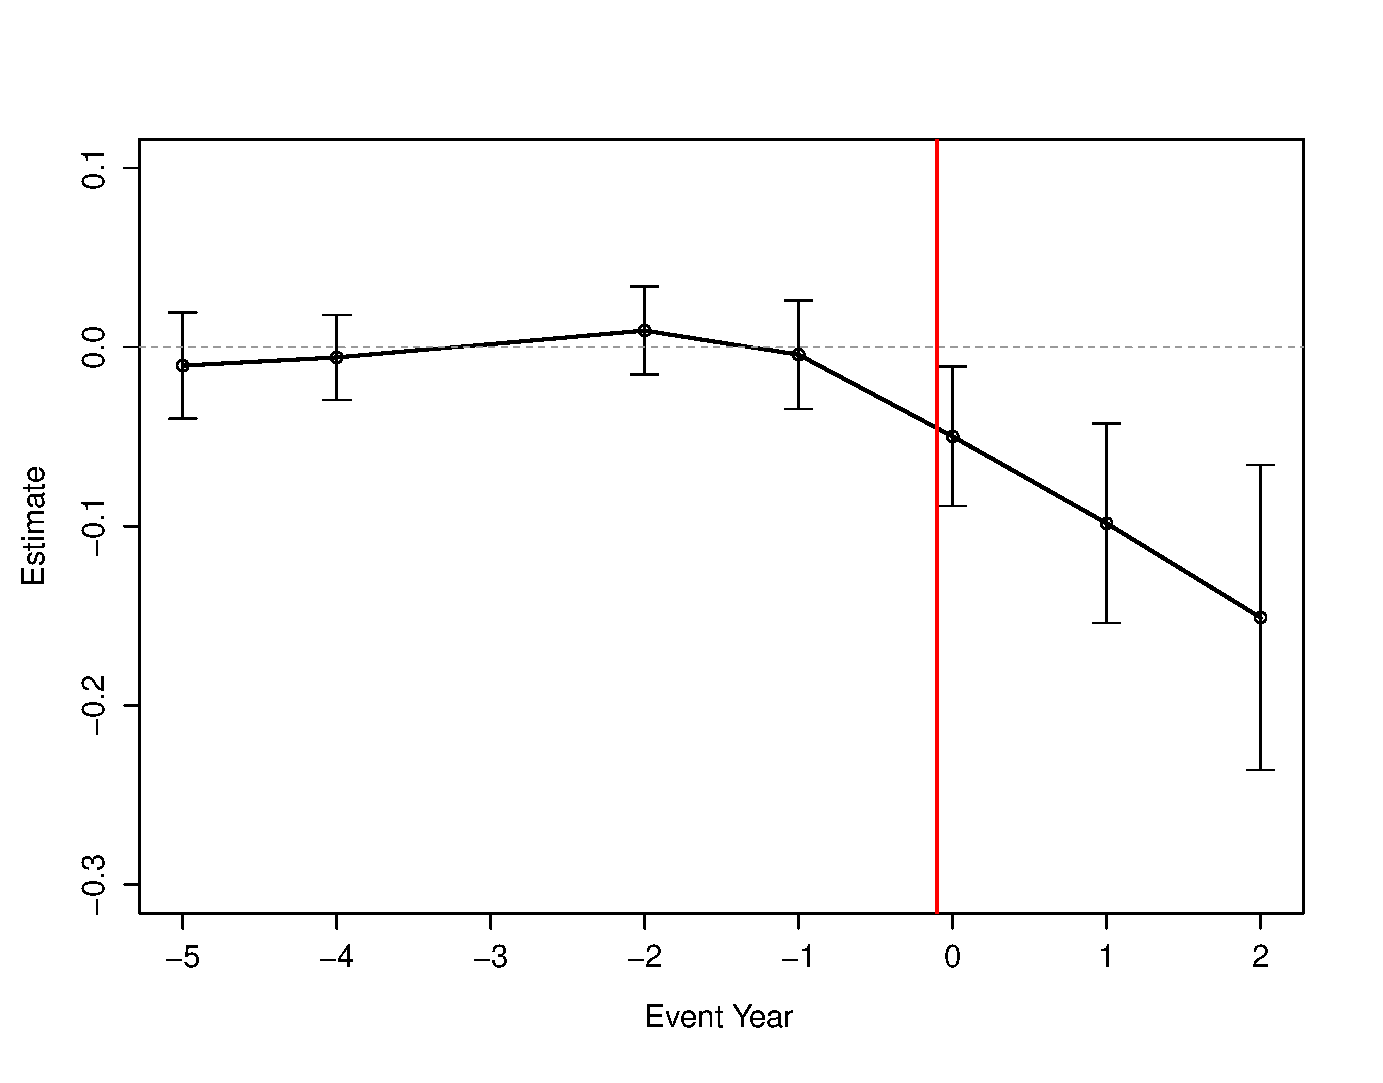
\includegraphics[scale=0.33]{\sdidloc/figures/Event1519treat.eps}
  \caption{Full Event Study: Treatment}
  \label{Sfig:eventT}
\end{subfigure}%
\begin{subfigure}{.5\textwidth}
  \centering
  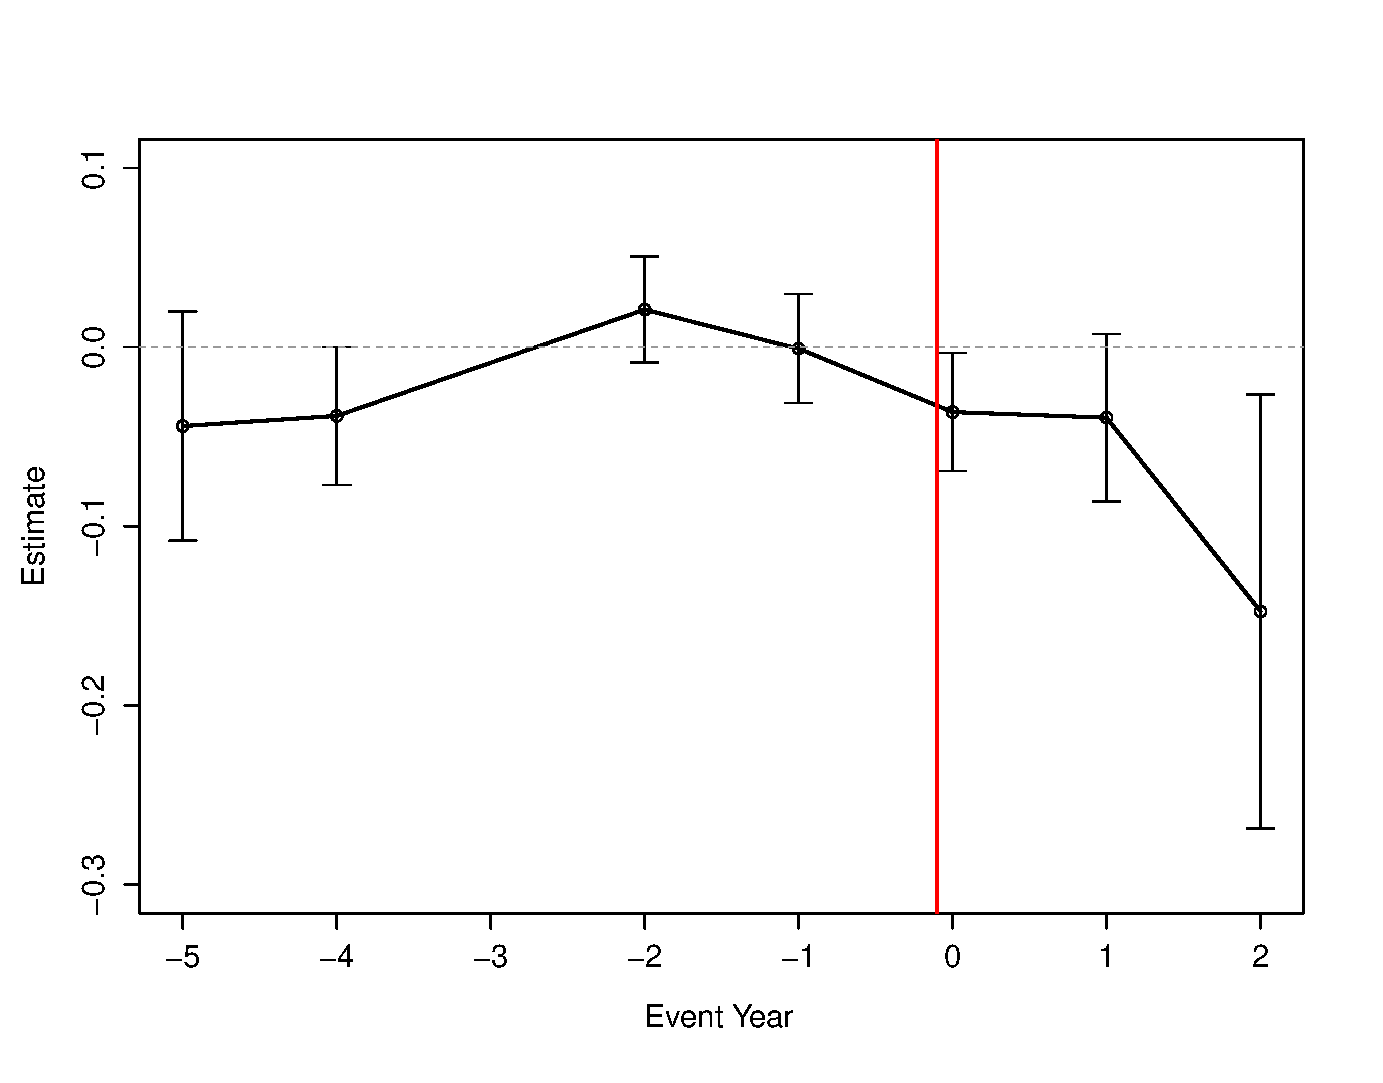
\includegraphics[scale=0.33]{\sdidloc/figures/Event1519close.eps}
  \caption{Full Event Study: Close to Treatment}
  \label{Sfig:eventC}
\end{subfigure}
\caption{Chile Event Study for ATT and ATC}
\label{Sfig:eventStudy}
\end{center}
\floatfoot{\textsc{Notes to figure}: In each figures the horizontal dotted line 
represents an effect size of 0.  The vertical solid line represents the first 
birth cohort affected by the reform.  Each point on the plot represents the
effect of living in a treatment (panel A) or close to treatment (panel B) 
municipality $x$ years before or after the reform took effect.  Error bars 
represent 95\% confidence intervals of these estimates.}
\end{figure}


\section{Additional Details: 2007 Mexico Abortion Reform}
\label{Sscn:MAbort}
On April 26, 2007 the legislative assembly of the Federal District of Mexico
City (Mexico DF), voted to legalise abortion (termed legal interruption of
pregnancy) whenever requested by the woman up to 12 weeks of gestation,
reforming article 144 of the penal code of Mexico DF. This immediately 
permitted women from DF to request (free) legal interruption of pregnancy in 
public health clinics, with a large influx of requests 
\citep{Contrerasetal2011}. On August 29, 2008 this decision was ratified by the 
Supreme Court of Mexico.

As well as decriminalising abortion, the law dictated that Mexico DF Department
of Health facilities offer free abortion to residents of DF, and on a variable
pay scale for women from other areas of the country \citep{Beckeretal2013}. 
Prior to the April 2006 findings, abortion was illegal in Mexico DF (and all of
Mexico) in all but a very limited set of circumsances (depending on the state,
these circumstances include none, some, or all of rape, fetal inviability or 
grave danger to the health of the mother).  Along with free pregnancy 
terminations at Ministry of Health clinics, following the reform private 
health centres were also allowed to provide abortions.  
%Finally, in 2011, the
%Federal Commission of Protection Against Sanitary Risk (COFEPRIS) authorised
%the sale of Mifepristona...

Abortion services were widely accessed following the reform.  Between April 
of 2007 and the end of 2011, 80,000 abortions were performed.  These were 
accessed by women over the entire age range of the fertility distribution,
reasonably closely mirroring mother's age at birth in birth data (figure
\ref{SFig:MexBirthAbort}), though with a slightly higher rate for younger
women.  Prior to April 2007 very few legal abortions were performed (n line
with the restrictions listed above).  Between 2001 and 2007 only 62 legal
abortions were performed, though clandestine abortion was very common 
\citep{Beckeretal2013}.  Further details regarding the reform, demand and
subsequent state decisions can be found in \citep{Beckeretal2013}, and 
references therein.

\section{The Chilean Legislative Environment and the Adoption of Emergency Contraception}
\label{TEENscn:applegislate}
Discussions surrounding the introduction of emergency contraception in Chile
have taken place since at least 1996, when the Chilean Institute of 
Reproductive Medicine (ICMER for its initials in Spanish) proposed the use of
this method to avoid undesired pregnancies in a country where abortion was
entirely outlawed \citep{Dides2009}.  However, the first legislative attention
given to this matter occurred when the Chilean Institute of Public Health 
emitted a resolution allowing
for the production and sale of `Postinol', a drug containing levonogestrel by a
Chilean laboratory in 2001.  The Constitionality of this was quickly 
challenged, and the drug was prohibited by the Supreme Court.

The emergency contraceptive pill again entered legislative attention in 2004,
following the Ministry of Health's publication of a guide suggesting that 
emergency contraception be used following cases of rape.  Following this in 
2005, the Subsecretary of Health Dr.\ Antonio Infante announced that emergency
contraception would be freely available to \emph{all} women who requested it,
however the President of Chile and the Ministry of Health later declared that
this was not the case, leading to removal of the Subsecretary from office.

In November of 2005, the Supreme Court of Chile provided the first 
constitutional support for the emergency contraceptive pill, voting 5-0 to
reverse the decision taken in 2001, allowing emergency contraception to be
provided in the case that the mother's life was in danger.  Once again however,
this finding was challenged shortly thereafter.  The same non-governmental 
institution which had earlier raised a case against ICMER, now challenged the 
private commercial laboratory in charge of producing and distributing the drug.  
However, before this case could reach court, this laboratory voluntarily gave 
up their license to produce the drug, in a three line statement issued by the
General Director of the company on February 14, 2006 \citep{CasasBecerra2008}.

In the same year, a group of 36 parliamentary deputies from conservative 
parties raised a case with the Constitional Tribunal, claiming that the 
provision of the emergency contraceptive pill contravened the ``National Laws
for the Regulation of Fertility'', a set of rules issued by the Ministry of
Health.  This case was only resolved in 2008, with the Constitional Tribunal's
finding in favour of this group, hence making illegal any provision by 
hospitals or health centres controlled by the Ministry of Health (and hence
under the jurisdiction of the National Fertility Laws).  Fundamentally however,
this left the door open for Municipal health centres to distribute the pill
freely to women.  These Municipal Health Centres are run under the directive
of the elected mayor of each Municipality, leaving all remaining legislation 
regarding the distribution of the pill up to the 346 mayors in Chile.

In this study I examine the period surrounding this 2008 legislation as the 
cutoff of interest.  However, even after this finding the emergency 
contraceptive pill has not been far from legislative action, with a number of
other cases raised.  These cases never entirely threatened the continuity of
supply of the morning after pill by municipalities, however did cause some
confusion for mayors and municipal health bodies in determining whether or not
they were legally allowed to prescribe the contraceptive.  These cases also
resulted in the passing of a number of laws and standards.  Most importantly,
they resulted in national Law 20.418 which ``creates standards for information,
guidance and regulatory services in fertility'' (author's translation), and 
the passing of a decree on March 3, 2013, which makes obligatory the provision
of the morning after pill to women of any age in any health centre in Chile.  
This became operative on May 28, 2013, meaning that---at least officially---%
there are no longer any restrictions in place in the country.

\section{Appendix Figures}
\label{Sscn:Agraphs}

\begin{figure}[h!]
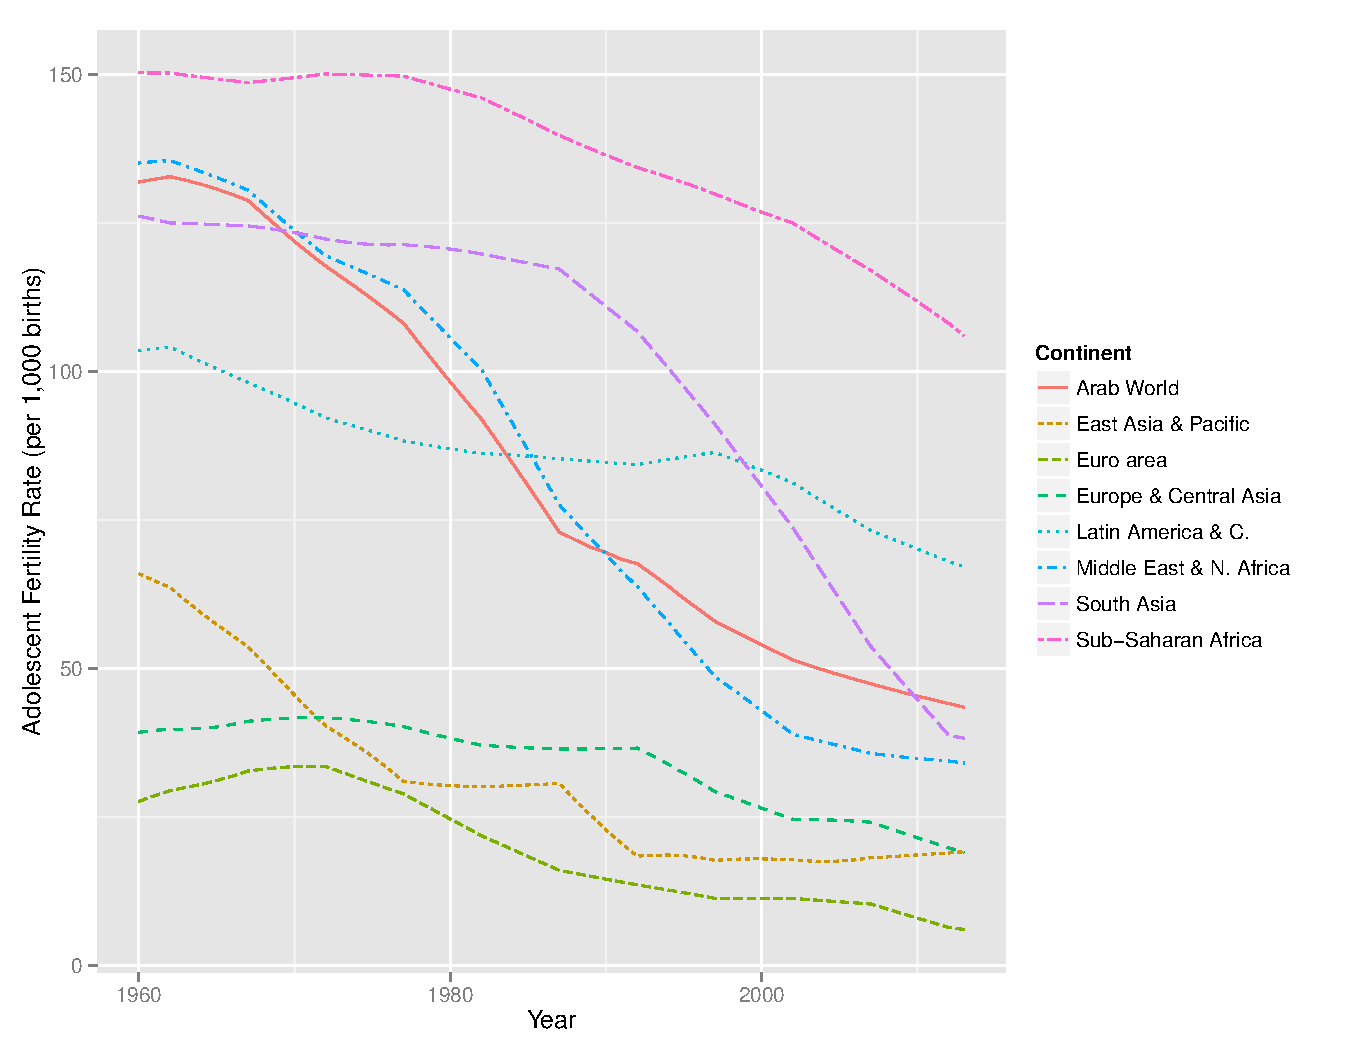
\includegraphics[scale=0.5]{Continents.pdf}
\caption{Adolescent Pregnancy Rates in Latin America and the World}
\label{SFig:continents}
\vspace{2mm}
\end{figure}

\begin{figure}[h!]
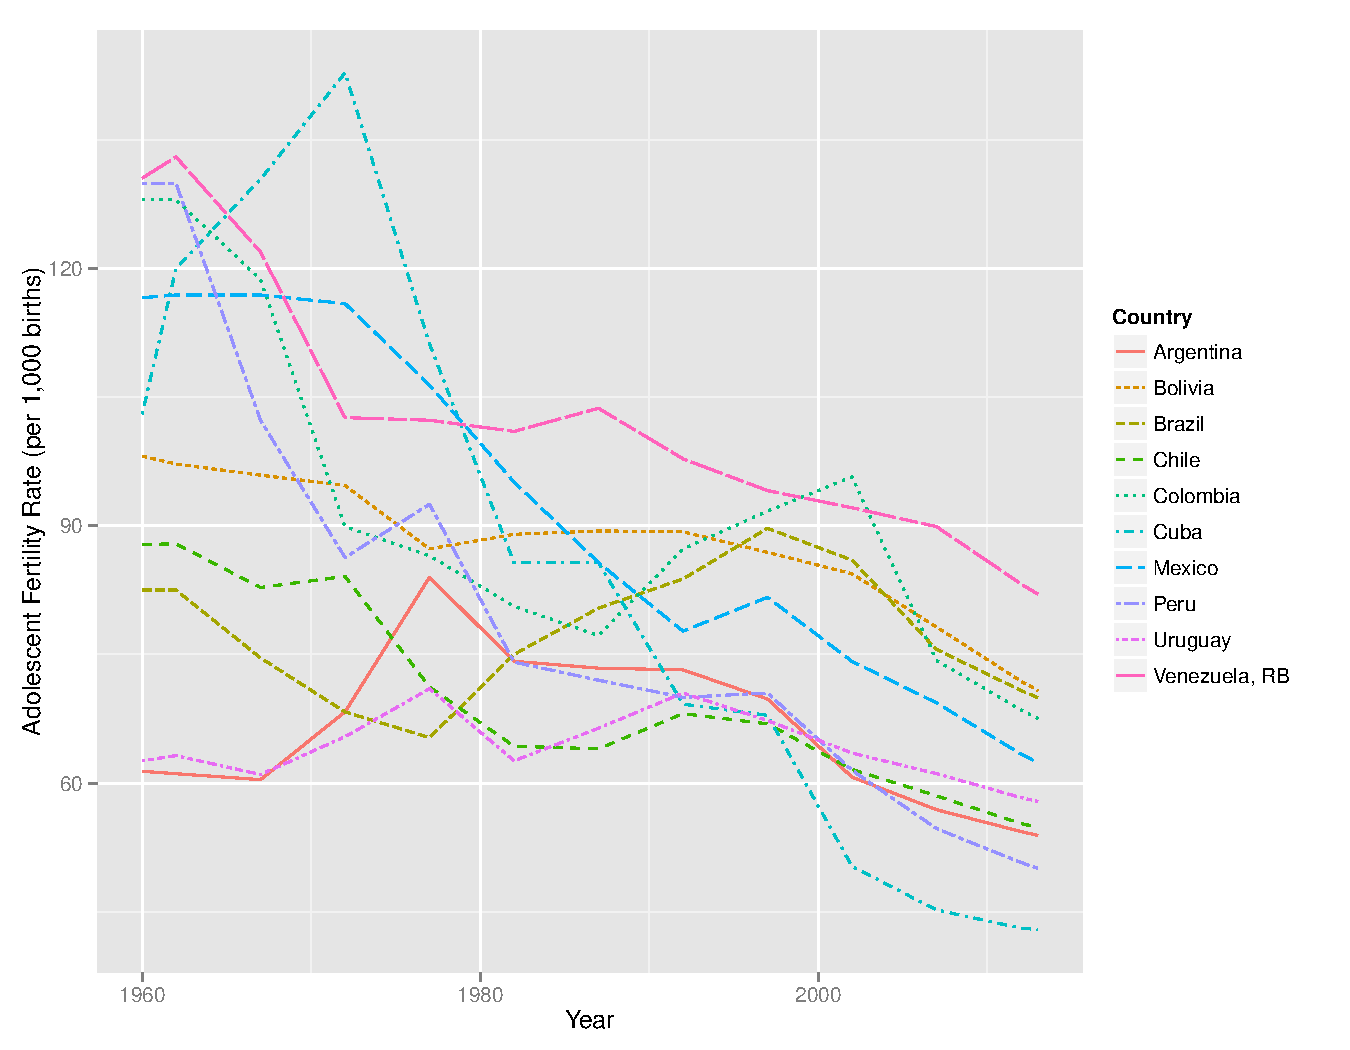
\includegraphics[scale=0.5]{Countries.pdf}
\caption{Adolescent Pregnancy Rates In Various Latin American Countries}
\label{SFig:countries}
\vspace{2mm}
\floatfoot{
\textsc{Notes to figures \ref{SFig:continents}-\ref{SFig:countries}}: Adolescent 
pregnancy rates come from the World Bank
Data Bank, and are expressed as number of births per 1,000 15-19 year-old women.}
\end{figure}


\begin{figure}[h!]
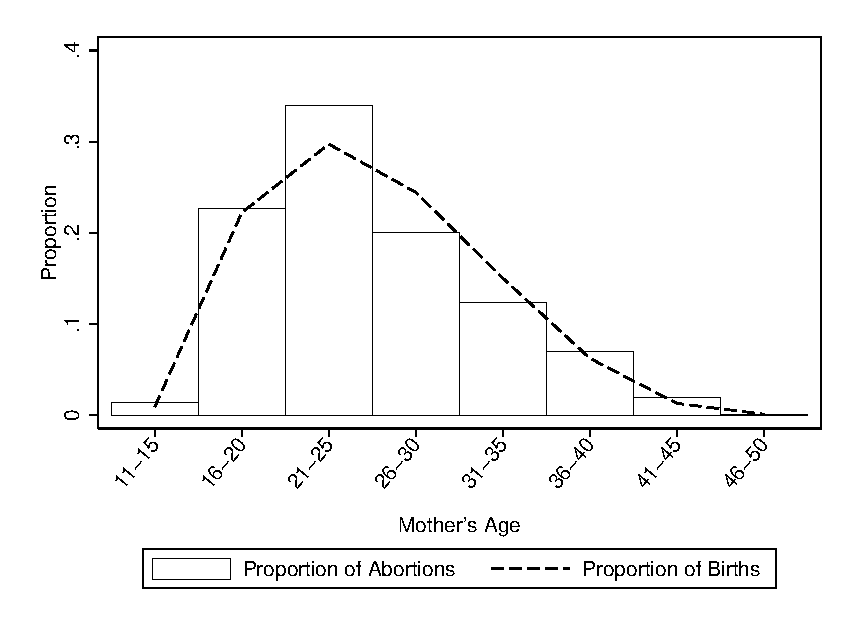
\includegraphics[scale=0.76]{\sdidloc/figures/birthDescriptives.eps}
\caption{Birth and Abortion Descriptives: Mexico}
\label{SFig:MexBirthAbort}
\vspace{2mm}
\floatfoot{
\textsc{Notes to figure}: Total births are plotted between 2001 and 2010.
Abortions are plotted from the date of reform (April 26, 2007) until 2011.
The total quantity of births is 22.20 million (all of Mexico), and total
abortions are 69,861 (Mexico DF only).  Births are calculated from 
administrative data (INEGI) and abortions from administrative data (Secretary
of Health, Mexico DF).}
\end{figure}


\begin{figure}[htpb!]
\caption{Estimate of Average Treatment Effect when Controlling for Travel Time}
\label{Sfig:ATTTime}
\vspace{-8mm}
\includegraphics[scale=0.55]{\sdidloc/figures/Dist1519_TIME.eps}
\end{figure}

\clearpage
\newpage
\section{Appendix Tables}
\label{Sscn:Atables}
\input{\sdidloc/tables/AgeGroupN2.tex}
\input{\sdidloc/tables/AgeGroupN3.tex}
\input{\sdidloc/tables/spill2034Chile.tex}
\input{\sdidloc/tables/spill3549Chile.tex}
